% ===========================================================================
%  BÁO CÁO ĐỒ ÁN MÔN HỌC — CÔNG NGHỆ WEB VÀ ỨNG DỤNG
%  Đề tài: SYNERGIT — Ứng dụng quản lý quy trình phát triển phần mềm
%          tích hợp quản lý mã nguồn dự án áp dụng kiến trúc Microservices
%
%  Biên dịch:  tectonic main.tex      (khuyến nghị)
%          hoặc xelatex main.tex  (chạy 2–3 lần để cập nhật mục lục)
%  KHÔNG dùng pdflatex (tài liệu dùng fontspec/XeLaTeX cho tiếng Việt).
% ===========================================================================
\documentclass[13pt,a4paper,oneside]{report}
% ===========================================================================
%  preamble.tex — Cấu hình gói, font, kiểu trình bày cho báo cáo Synergit
%  Biên dịch bằng XeLaTeX / Tectonic (hỗ trợ tiếng Việt qua fontspec).
% ===========================================================================

\usepackage{fontspec}
% Dùng font mặc định của LaTeX: Latin Modern (Computer Modern) — hỗ trợ đầy đủ
% glyph tiếng Việt. fontspec tự nạp Latin Modern khi không chỉ định font khác.
\setmainfont{lmroman10-regular.otf}[
  BoldFont = lmroman10-bold.otf,
  ItalicFont = lmroman10-italic.otf,
  BoldItalicFont = lmroman10-bolditalic.otf ]
\setsansfont{lmsans10-regular.otf}[
  BoldFont = lmsans10-bold.otf,
  ItalicFont = lmsans10-oblique.otf,
  BoldItalicFont = lmsans10-boldoblique.otf ]
\setmonofont{lmmonolt10-regular.otf}[
  BoldFont = lmmonolt10-bold.otf,
  ItalicFont = lmmonolt10-oblique.otf,
  BoldItalicFont = lmmonolt10-boldoblique.otf, Scale = 0.95 ]

\usepackage{geometry}
\geometry{a4paper, left=3cm, right=2cm, top=2cm, bottom=2cm}

\usepackage{amsmath,amssymb}
\usepackage{graphicx}
\usepackage{xcolor}
\usepackage{colortbl}
\usepackage{array}
\usepackage{longtable}
\usepackage{booktabs}
\usepackage{tabularx}
\usepackage{multirow}
\usepackage{enumitem}
\usepackage{ragged2e}
\usepackage{float}
\usepackage{caption}
\usepackage{titlesec}
\usepackage{titletoc}
\usepackage{fancyhdr}
\usepackage{setspace}
\usepackage{parskip}
\usepackage[hidelinks]{hyperref}
\usepackage{xurl}   % cho phép URL dài tự ngắt dòng
\usepackage{tikz}
\usetikzlibrary{shapes.geometric, arrows.meta, positioning, fit, calc, backgrounds, matrix}
\usepackage{tcolorbox}

% --- Màu chủ đề (Synergit: xanh lam GitHub-ish) -----------------------------
\definecolor{sgBlue}{HTML}{0969DA}
\definecolor{sgInk}{HTML}{1F2328}
\definecolor{sgCream}{HTML}{F6F8FA}
\definecolor{sgLine}{HTML}{D0D7DE}
\definecolor{sgAccent}{HTML}{2DA44E}
\colorlet{bkCream}{sgCream}
\colorlet{bkLine}{sgLine}
\colorlet{bkBrown}{sgInk}
\definecolor{codebg}{HTML}{F4F4F4}
\definecolor{codekw}{HTML}{0969DA}
\definecolor{codecm}{HTML}{6A737D}
\definecolor{codestr}{HTML}{1B7A43}

% Kiểu dùng chung cho các sơ đồ ERD theo schema
\tikzset{
  erdent/.style={draw=sgBlue, fill=sgCream, rounded corners, align=left,
                 inner sep=4pt, font=\scriptsize, text width=3.05cm},
  erdext/.style={draw=sgLine, dashed, fill=white, rounded corners, align=center,
                 inner sep=4pt, font=\scriptsize\itshape, text width=2.6cm},
  erdrel/.style={draw=sgLine, thick},
  erdsoft/.style={draw=sgLine, thick, dashed},
  erdcard/.style={font=\scriptsize, text=sgBlue, fill=white, inner sep=1pt},
}
\tcbuselibrary{skins, breakable}
\usepackage{listings}

% --- Cỡ chữ 13pt, giãn dòng 1.5 (chuẩn báo cáo đồ án) -----------------------
\renewcommand{\normalsize}{\fontsize{13pt}{19.5pt}\selectfont}
\normalsize
\setstretch{1.42}

% --- Canh lề hai bên, hạn chế ngắt từ tiếng Việt ---------------------------
\justifying
\hyphenpenalty=8000
\tolerance=2000
\setlength{\emergencystretch}{3em}

% --- Nhãn tiếng Việt cho Hình / Bảng / Mục lục -----------------------------
\captionsetup{labelsep=colon, font=small, labelfont=bf}
\captionsetup[figure]{name=Hình}
\captionsetup[table]{name=Bảng}
\renewcommand{\chaptername}{Chương}
\renewcommand{\contentsname}{MỤC LỤC}
\renewcommand{\listfigurename}{MỤC LỤC HÌNH ẢNH}
\renewcommand{\listtablename}{MỤC LỤC BẢNG}
\renewcommand{\bibname}{TÀI LIỆU THAM KHẢO}
\renewcommand{\figurename}{Hình}
\renewcommand{\tablename}{Bảng}

% --- Đánh số Hình/Bảng theo chương -----------------------------------------
\usepackage{chngcntr}
\counterwithin{figure}{chapter}
\counterwithin{table}{chapter}

% --- Kiểu tiêu đề Chương / Mục ---------------------------------------------
\titleformat{\chapter}[display]
  {\centering\bfseries\fontsize{15pt}{18pt}\selectfont}
  {\MakeUppercase{\chaptertitlename}\ \thechapter}
  {6pt}
  {\MakeUppercase}
\titlespacing*{\chapter}{0pt}{0pt}{18pt}

\titleformat{\section}
  {\bfseries\fontsize{13.5pt}{16pt}\selectfont}{\thesection.}{0.5em}{}
\titleformat{\subsection}
  {\bfseries\itshape\fontsize{13pt}{16pt}\selectfont}{\thesubsection.}{0.5em}{}
\titleformat{\subsubsection}
  {\itshape\fontsize{13pt}{16pt}\selectfont}{\thesubsubsection.}{0.5em}{}
\titlespacing*{\section}{0pt}{10pt}{4pt}
\titlespacing*{\subsection}{0pt}{8pt}{3pt}
\titlespacing*{\subsubsection}{0pt}{6pt}{3pt}

% --- Header / footer (số trang góc dưới) -----------------------------------
\pagestyle{fancy}
\fancyhf{}
\renewcommand{\headrulewidth}{0pt}
\fancyfoot[C]{\thepage}
\fancypagestyle{plain}{\fancyhf{}\fancyfoot[C]{\thepage}\renewcommand{\headrulewidth}{0pt}}

% --- Danh sách gọn hơn ------------------------------------------------------
\setlist[itemize]{leftmargin=1.4em, topsep=2pt, itemsep=1pt, parsep=0pt}
\setlist[enumerate]{leftmargin=1.8em, topsep=2pt, itemsep=1pt, parsep=0pt}

% --- Kiểu khối mã nguồn -----------------------------------------------------
\lstdefinestyle{sg}{
  backgroundcolor=\color{codebg},
  basicstyle=\ttfamily\footnotesize,
  keywordstyle=\color{codekw}\bfseries,
  commentstyle=\color{codecm}\itshape,
  stringstyle=\color{codestr},
  numbers=left, numberstyle=\tiny\color{codecm}, numbersep=8pt,
  breaklines=true, showstringspaces=false, tabsize=2,
  frame=single, rulecolor=\color{sgLine},
  framexleftmargin=4pt, xleftmargin=14pt, aboveskip=8pt, belowskip=6pt,
  columns=fullflexible, keepspaces=true,
}
\lstset{style=sg}
\lstdefinelanguage{Go}{
  keywords={func,package,import,type,struct,interface,map,chan,go,defer,return,if,else,for,range,switch,case,default,var,const,nil,error,select},
  ndkeywords={string,int,int64,bool,uint,byte,UUID,context},
  sensitive=true, comment=[l]{//}, morecomment=[s]{/*}{*/},
  morestring=[b]", morestring=[b]`,
}
\lstdefinelanguage{TypeScript}{
  keywords={const,let,var,function,async,await,return,if,else,for,of,in,while,
            import,export,from,type,interface,class,extends,implements,new,
            public,private,readonly,as,enum,void,null,undefined,true,false},
  ndkeywords={string,number,boolean,Promise,Record,Array,Partial},
  sensitive=true, comment=[l]{//}, morecomment=[s]{/*}{*/},
  morestring=[b]", morestring=[b]', morestring=[b]`,
}

% --- Lệnh chèn ảnh placeholder (chờ ảnh chụp màn hình thật) -----------------
% \phimg{<caption>}{<chiều cao>}  — ví dụ \phimg{Giao diện trang Home}{6cm}
\newcommand{\phimg}[2]{%
  \begin{figure}[H]\centering
  \begin{tcolorbox}[width=0.88\linewidth, height=#2, halign=center, valign=center,
      colback=sgCream, colframe=sgLine, sharp corners, boxrule=0.6pt,
      before skip=4pt, after skip=2pt]
      {\color{sgInk}\itshape [\,Ảnh minh hoạ:\ #1\,]\\[4pt]\footnotesize (chèn ảnh chụp màn hình thật tại đây)}
  \end{tcolorbox}
  \caption{#1}
  \end{figure}}

% --- Lệnh chèn ảnh "thông minh" (skeleton) ---------------------------------
% \figauto[<nhãn>]{<đường dẫn file>}{<caption>}{<chiều cao tối đa>}
%   • Nếu file ảnh TỒN TẠI  -> tự chèn ảnh (giới hạn theo bề rộng & chiều cao).
%   • Nếu CHƯA có file       -> hiện khung placeholder ghi rõ tên file cần bỏ vào.
\newcommand{\figautolabel}{}
\newcommand{\figauto}[4][]{%
  \renewcommand{\figautolabel}{#1}%
  \begin{figure}[H]\centering
  \IfFileExists{#2}{%
    \includegraphics[width=0.95\linewidth, height=\dimexpr#4*13/10\relax, keepaspectratio]{#2}%
  }{%
    \begin{tcolorbox}[width=0.88\linewidth, height=#4, halign=center, valign=center,
        colback=sgCream, colframe=sgLine, sharp corners, boxrule=0.6pt,
        before skip=4pt, after skip=2pt]
        {\color{sgInk}\itshape [\,Đặt ảnh vào:\ \texttt{#2}\,]\\[4pt]
         \footnotesize #3}
    \end{tcolorbox}%
  }%
  \caption{#3}%
  \ifx\figautolabel\empty\else\label{#1}\fi
  \end{figure}}

% --- Tiêu đề trang phụ (không đánh số chương) cho phần đầu ------------------
\newcommand{\plainheading}[1]{%
  \par\vspace{6pt}\begin{center}\bfseries\fontsize{15pt}{18pt}\selectfont\MakeUppercase{#1}\end{center}\vspace{4pt}}

% --- Bảng đặc tả Usecase ----------------------------------------------------
% Dùng:  \begin{ucspec}{nhãn}{Tiêu đề bảng}  ... các dòng "Trường & Giá trị \\\hline" ... \end{ucspec}
\newenvironment{ucspec}[2]{%
  \renewcommand{\arraystretch}{1.25}\small
  \begin{longtable}{|>{\bfseries\raggedright\arraybackslash}p{3.4cm}|p{10.3cm}|}
  \caption{#2}\label{#1}\\
  \hline\endfirsthead
  \hline\multicolumn{2}{|r|}{\textit{(tiếp theo)}}\\\hline\endhead
}{%
  \end{longtable}\normalsize}

% --- Bảng đặc tả chi tiết bảng dữ liệu --------------------------------------
% Dùng:  \begin{dbtable}{nhãn}{Tiêu đề}  ... "STT & trường & kiểu & mô tả \\\hline" ... \end{dbtable}
\newenvironment{dbtable}[2]{%
  \renewcommand{\arraystretch}{1.2}\small
  \begin{longtable}{|c|>{\ttfamily}p{3.5cm}|>{\ttfamily}p{2.8cm}|p{5.3cm}|}
  \caption{#2}\label{#1}\\
  \hline\rowcolor{sgCream}
  \textbf{STT} & \normalfont\textbf{Tên trường} & \normalfont\textbf{Kiểu dữ liệu} & \textbf{Mô tả}\\\hline
  \endfirsthead
  \hline\rowcolor{sgCream}
  \textbf{STT} & \normalfont\textbf{Tên trường} & \normalfont\textbf{Kiểu dữ liệu} & \textbf{Mô tả}\\\hline
  \endhead
}{%
  \end{longtable}\normalsize}


% ---------------------------------------------------------------------------
%  THÔNG TIN TRANG BÌA  — SỬA CÁC GIÁ TRỊ DƯỚI ĐÂY CHO NHÓM CỦA BẠN
% ---------------------------------------------------------------------------
\newcommand{\BoGiaoDuc}{BỘ GIÁO DỤC VÀ ĐÀO TẠO}
\newcommand{\TruongDH}{TRƯỜNG ĐẠI HỌC CÔNG NGHỆ THÔNG TIN}
\newcommand{\Khoa}{KHOA CÔNG NGHỆ PHẦN MỀM}
\newcommand{\TenMonHoc}{ĐỒ ÁN 2}
\newcommand{\TenDeTaiNgan}{SYNERGIT}
\newcommand{\TenDeTai}{ỨNG DỤNG QUẢN LÝ QUY TRÌNH PHÁT TRIỂN PHẦN MỀM\\ TÍCH HỢP QUẢN LÝ MÃ NGUỒN DỰ ÁN ÁP DỤNG\\ KIẾN TRÚC MICROSERVICES}
% Lưu ý: thêm học vị (ThS./TS.) trước tên GVHD nếu cần.
\newcommand{\GVHD}{TS. Huỳnh Minh Đức}
\newcommand{\Lop}{SE122.Q21}
% Sinh viên thực hiện (đồ án 1 người — chỉnh sửa cho phù hợp nếu là nhóm 2 người)
\newcommand{\SVMot}{Nguyễn Phúc Thịnh}
\newcommand{\MSSVMot}{23521503}
\newcommand{\DiaDiemThoiGian}{Tp.\ Hồ Chí Minh, tháng 6 năm 2026}

\begin{document}

% =========================== TRANG BÌA =====================================
\begin{titlepage}
\begin{tikzpicture}[remember picture, overlay]
  \draw[line width=0.8pt]
    ([xshift=0.8cm,yshift=-0.8cm]current page.north west)
    rectangle
    ([xshift=-0.8cm,yshift=0.8cm]current page.south east);
  \draw[line width=0.4pt]
    ([xshift=0.95cm,yshift=-0.95cm]current page.north west)
    rectangle
    ([xshift=-0.95cm,yshift=0.95cm]current page.south east);
\end{tikzpicture}
\centering
\setstretch{1.3}
{\bfseries\fontsize{14pt}{17pt}\selectfont \BoGiaoDuc\par}
{\bfseries\fontsize{14pt}{17pt}\selectfont \TruongDH\par}
{\bfseries\fontsize{14pt}{17pt}\selectfont \Khoa\par}
\vspace{1.0cm}

% Logo trường — tự hiện khi có file image/logo-truong.png
\IfFileExists{image/logo-truong.png}{%
  \includegraphics[height=3.4cm, keepaspectratio]{image/logo-truong.png}%
}{%
  \IfFileExists{../latex/image/logo-truong.png}{%
    \includegraphics[height=3.4cm, keepaspectratio]{../latex/image/logo-truong.png}%
  }{%
    \begin{tcolorbox}[width=3.4cm, height=3.4cm, halign=center, valign=center,
       colback=bkCream, colframe=bkLine, sharp corners, boxrule=0.6pt]
       {\color{bkBrown}\itshape \footnotesize Đặt logo:\\ \texttt{\scriptsize image/logo-truong.png}}
    \end{tcolorbox}%
  }%
}

\vspace{1.0cm}
{\bfseries\fontsize{18pt}{22pt}\selectfont BÁO CÁO\par}
\vspace{0.3cm}
{\bfseries\fontsize{16pt}{20pt}\selectfont \TenMonHoc\par}
\vspace{1.4cm}

{\bfseries\fontsize{22pt}{27pt}\selectfont \TenDeTaiNgan\par}
\vspace{0.35cm}
{\bfseries\fontsize{17pt}{22pt}\selectfont \TenDeTai\par}

\vspace{1.4cm}
\begin{minipage}{0.80\textwidth}
\bfseries\fontsize{14pt}{20pt}\selectfont
\begin{tabular}{@{}ll@{}}
Giảng viên hướng dẫn & : \GVHD\\[5pt]
Lớp & : \Lop\\[5pt]
Sinh viên thực hiện & : \SVMot\ -- \MSSVMot\\[5pt]
\end{tabular}
\end{minipage}

\vfill
{\bfseries\fontsize{13pt}{16pt}\selectfont \DiaDiemThoiGian\par}
\end{titlepage}

% =========================== PHẦN ĐẦU ======================================
\pagenumbering{roman}

% ====================== BẢNG PHÂN CÔNG CÔNG VIỆC ===========================
\plainheading{Bảng phân công công việc}

\noindent
\renewcommand{\arraystretch}{1.35}
\begin{longtable}{|>{\centering\arraybackslash}m{1.8cm}|>{\centering\arraybackslash}m{2.8cm}|>{\raggedright\arraybackslash}m{6.2cm}|>{\centering\arraybackslash}m{1.9cm}|}
\hline
\rowcolor{sgCream}
\multicolumn{1}{|c|}{\textbf{MSSV}} & \multicolumn{1}{c|}{\textbf{Họ và tên}} & \multicolumn{1}{c|}{\textbf{Nhiệm vụ}} & \textbf{Mức độ đóng góp}\\
\hline
\endhead
\MSSVMot & \SVMot &
1. Tổng phụ trách: lên kế hoạch, quản lý tiến độ, tạo repo và quản lý issue/ticket.\newline
2. Backend (Go + Gin): module xác thực, repo \& git operations, pull request, issue, insights, gateway.\newline
3. Frontend (React + TypeScript + Vite): toàn bộ giao diện người dùng.\newline
4. Thiết kế cơ sở dữ liệu, kiến trúc microservices.\newline
5. Triển khai (Docker, CI/CD) và viết báo cáo. & 100\% \\
\hline
\end{longtable}
\clearpage

% ====================== LỜI CẢM ƠN =========================================
\plainheading{Lời cảm ơn}

\hspace{1.2em}Lời đầu tiên, em xin gửi lời cảm ơn chân thành và lòng biết ơn sâu sắc đến Ban Giám hiệu và toàn thể quý Thầy Cô Trường Đại học Công nghệ Thông tin -- ĐHQG TP.HCM, đặc biệt là các Thầy Cô Khoa Công nghệ Phần mềm. Chính môi trường học tập năng động và những kiến thức quý báu mà quý Thầy Cô tận tâm truyền đạt đã tạo nên nền tảng vững chắc, tiếp thêm động lực để em không ngừng nỗ lực trong suốt quá trình học tập và nghiên cứu.

\hspace{1.2em}Đặc biệt, em xin bày tỏ lòng tri ân sâu sắc nhất đến thầy \GVHD, người đã dành rất nhiều thời gian, tâm huyết để trực tiếp hướng dẫn, theo sát và định hướng cho em trong suốt quá trình thực hiện đề tài \textit{``Synergit -- Ứng dụng quản lý quy trình phát triển phần mềm tích hợp quản lý mã nguồn dự án áp dụng kiến trúc Microservices''}. Những lời khuyên chuyên môn, sự chỉ dẫn tận tình về mặt kỹ thuật và những ý kiến đóng góp sửa chữa của Thầy đã giúp em tháo gỡ nhiều khó khăn, từ đó từng bước hoàn thiện đồ án này một cách tốt nhất.

\hspace{1.2em}Đề tài này hướng tới việc ứng dụng các kỹ thuật phân chia hệ thống theo Domain-Driven Design (DDD) để xây dựng một nền tảng quản lý mã nguồn (giống GitHub thu nhỏ) theo kiến trúc microservices. Đây là một chủ đề mang tính kỹ thuật cao, đòi hỏi không chỉ kiến thức về lập trình web mà còn cả về Git internals, kiến trúc hệ phân tán, mẫu thiết kế và bảo mật. Quá trình thực hiện vì thế là một hành trình học hỏi quý giá đối với em.

\hspace{1.2em}Tuy nhiên, do giới hạn về mặt thời gian cũng như năng lực và kinh nghiệm thực tế của em vẫn còn nhiều hạn chế, đồ án chắc chắn không thể tránh khỏi những thiếu sót. Em rất mong nhận được sự cảm thông, lượng thứ từ quý Thầy Cô. Đồng thời, em cũng hy vọng sẽ nhận được những ý kiến đóng góp quý báu từ Thầy và Hội đồng để sản phẩm được hoàn thiện hơn, giúp em rút ra được những bài học kinh nghiệm quý giá cho hành trình nghề nghiệp sau này.

\begin{flushright}
\textit{Trân trọng cảm ơn!}\\
\textit{Thành phố Hồ Chí Minh, tháng 6 năm 2026}\\
\textbf{Sinh viên thực hiện}\\
\SVMot
\end{flushright}
\clearpage


% --- Mục lục, mục lục bảng, mục lục hình ------------------------------------
\tableofcontents
\clearpage
\listoftables
\clearpage
\listoffigures
\clearpage
% ====================== DANH MỤC TỪ VIẾT TẮT ===============================
\plainheading{Danh mục từ viết tắt}
\addcontentsline{toc}{chapter}{DANH MỤC TỪ VIẾT TẮT}

\renewcommand{\arraystretch}{1.3}
\begin{longtable}{|>{\bfseries}p{2.8cm}|p{11.0cm}|}
\hline
\rowcolor{sgCream}
\multicolumn{1}{|c|}{\textbf{Từ viết tắt}} & \multicolumn{1}{c|}{\textbf{Diễn giải}}\\
\hline
\endfirsthead
\hline
\rowcolor{sgCream}
\multicolumn{1}{|c|}{\textbf{Từ viết tắt}} & \multicolumn{1}{c|}{\textbf{Diễn giải}}\\
\hline
\endhead
API    & Application Programming Interface -- giao diện lập trình ứng dụng.\\\hline
CI/CD  & Continuous Integration / Continuous Deployment -- tích hợp và triển khai liên tục.\\\hline
CRUD   & Create -- Read -- Update -- Delete -- các thao tác cơ bản trên dữ liệu.\\\hline
CSDL   & Cơ sở dữ liệu.\\\hline
DAG    & Directed Acyclic Graph -- đồ thị có hướng không chu trình (cấu trúc lịch sử commit của Git).\\\hline
DDD    & Domain-Driven Design -- thiết kế phần mềm theo miền nghiệp vụ.\\\hline
DTO    & Data Transfer Object -- đối tượng truyền dữ liệu giữa các tầng.\\\hline
ERD    & Entity -- Relationship Diagram -- sơ đồ thực thể -- quan hệ.\\\hline
FK     & Foreign Key -- khoá ngoại.\\\hline
FSM    & Finite State Machine -- máy trạng thái hữu hạn.\\\hline
HMAC   & Hash-based Message Authentication Code -- mã xác thực thông điệp dùng băm.\\\hline
HTTP / HTTPS & HyperText Transfer Protocol (Secure) -- giao thức truyền siêu văn bản (bảo mật).\\\hline
JSON   & JavaScript Object Notation -- định dạng trao đổi dữ liệu.\\\hline
JSONB  & JSON Binary -- kiểu dữ liệu JSON nhị phân của PostgreSQL.\\\hline
JWT    & JSON Web Token -- chuẩn token dùng cho xác thực.\\\hline
PK     & Primary Key -- khoá chính.\\\hline
PR     & Pull Request -- yêu cầu trộn nhánh / yêu cầu hợp nhất mã nguồn.\\\hline
RBAC   & Role-Based Access Control -- kiểm soát truy cập theo vai trò.\\\hline
REST   & Representational State Transfer -- kiến trúc giao tiếp web phổ biến.\\\hline
SCM    & Source Code Management -- quản lý mã nguồn.\\\hline
SHA-1  & Secure Hash Algorithm 1 -- thuật toán băm 160-bit (Git dùng làm định danh đối tượng).\\\hline
SPA    & Single Page Application -- ứng dụng web một trang.\\\hline
SQL    & Structured Query Language -- ngôn ngữ truy vấn dữ liệu.\\\hline
SSR    & Server-Side Rendering -- kết xuất giao diện phía máy chủ.\\\hline
UI / UX & User Interface / User Experience -- giao diện / trải nghiệm người dùng.\\\hline
URL    & Uniform Resource Locator -- địa chỉ tài nguyên trên Internet.\\\hline
UUID   & Universally Unique Identifier -- định danh duy nhất toàn cục.\\\hline
VCS    & Version Control System -- hệ thống quản lý phiên bản.\\\hline
\end{longtable}
\clearpage


% =========================== NỘI DUNG =======================================
\pagenumbering{arabic}

% ====================== TÓM TẮT ĐỀ TÀI =====================================
\chapter*{TÓM TẮT ĐỀ TÀI}
\addcontentsline{toc}{chapter}{TÓM TẮT ĐỀ TÀI}

\hspace{1.2em}Trong xu thế phát triển phần mềm hiện đại, Git đã trở thành chuẩn không chính thức cho việc quản lý mã nguồn, kéo theo đó là sự thống trị của các nền tảng cộng tác như GitHub và GitLab. Các nền tảng này không chỉ đơn thuần lưu trữ kho mã nguồn mà còn tích hợp toàn bộ \textit{quy trình phát triển phần mềm}: pull request, code review, issue tracking, dòng thời gian sự kiện, thống kê đóng góp\ldots Tuy nhiên, các đội phát triển nội bộ tại Việt Nam thường gặp ba vấn đề: (1) phụ thuộc vào dịch vụ nước ngoài cho mã nguồn nhạy cảm, (2) chi phí cao khi cần nâng cấp tính năng cho đội nhiều thành viên, và (3) thiếu một mô hình tham khảo kiến trúc rõ ràng nếu muốn xây dựng hệ thống tương đương ở quy mô vừa.

\hspace{1.2em}Đề tài \textbf{``Synergit -- Ứng dụng quản lý quy trình phát triển phần mềm tích hợp quản lý mã nguồn dự án áp dụng kiến trúc Microservices''} được phát triển nhằm xây dựng một nền tảng quản lý mã nguồn và quy trình phát triển phần mềm theo mô hình GitHub thu nhỏ, có thể tự triển khai (self-hosted) cho đội phát triển nội bộ. Hệ thống cho phép người dùng đăng ký tài khoản, tạo repository công khai/riêng tư, push/pull mã nguồn qua giao thức Git Smart HTTP, duyệt cây thư mục, xem nội dung file và lịch sử commit, tạo và quản lý nhánh (branch). Đặc biệt, hệ thống hỗ trợ đầy đủ \textit{quy trình cộng tác}: tạo pull request, so sánh branch (diff), giải quyết xung đột (merge conflict), merge và revert, theo dõi event timeline; quản lý issue với label, assignee, comment; cùng các bảng phân tích thống kê (commit trend, language breakdown, contributor stats, contribution graph kiểu GitHub).

\hspace{1.2em}Về mặt kỹ thuật, Synergit được thiết kế và triển khai theo \textit{kiến trúc microservices} dựa trên triết lý ``Majestic Monolith + Strategic Services'' của GitHub: hệ thống gồm một API Gateway (cổng vào duy nhất), một dịch vụ \textit{Core} chứa phần lớn nghiệp vụ (auth, repo metadata, pull request, issue, label, collaborator, star), một dịch vụ \textit{GitStorage} chuyên xử lý các thao tác Git nặng I/O và sở hữu hệ thống tệp các kho mã nguồn, và một dịch vụ \textit{Insights} chuyên xử lý các tác vụ phân tích/CPU-bound. Các dịch vụ giao tiếp qua HTTP/REST, chia sẻ chung cơ chế xác thực JWT (HMAC), và mỗi dịch vụ sở hữu một schema PostgreSQL riêng (\texttt{core.*}, \texttt{insights.*}). Backend viết bằng Go (Gin), tận dụng Clean Architecture với các tầng \textit{domain}, \textit{port}, \textit{usecase}, \textit{adapter} -- nhờ đó việc tách dịch vụ chỉ là việc thay thế \textit{adapter} mà không làm thay đổi \textit{usecase}. Frontend là một ứng dụng React + Vite + TypeScript đơn lẻ.

\hspace{1.2em}Nội dung đồ án được trình bày gồm 5 chương:

\begin{itemize}
\item \textbf{Chương 1 -- Giới thiệu đề tài:} Bối cảnh, lý do chọn đề tài, mục tiêu nghiệp vụ và kỹ thuật, phạm vi chức năng, sơ đồ sitemap, công nghệ, môi trường và công cụ sử dụng.
\item \textbf{Chương 2 -- Cơ sở lý thuyết:} Kiến thức nền tảng về Git internals và giao thức Git Smart HTTP, công nghệ Frontend (React, TypeScript, Vite, Tailwind CSS), Backend (Go, Gin), hệ quản trị CSDL PostgreSQL, kiến trúc Microservices và Clean Architecture, cùng cơ chế xác thực JWT và bảo mật hệ thống.
\item \textbf{Chương 3 -- Phân tích thiết kế hệ thống:} Khảo sát hiện trạng, phân tích yêu cầu chức năng/phi chức năng, mô hình hoá bằng Usecase, kiến trúc microservices và thiết kế cơ sở dữ liệu (ERD, đặc tả bảng).
\item \textbf{Chương 4 -- Xây dựng website:} Thiết kế template giao diện và hiện thực hoá các trang chính của ứng dụng (đăng nhập, dashboard repository, code browser, pull request, issue, profile).
\item \textbf{Chương 5 -- Kết luận:} Tổng kết ưu điểm, hạn chế và đề xuất các hướng phát triển trong tương lai.
\end{itemize}
\clearpage
   % TÓM TẮT ĐỀ TÀI
\chapter{Giới thiệu đề tài}

Chương 1 tập trung giới thiệu tổng quan về đề tài \textit{``Synergit -- Ứng dụng quản lý quy trình phát triển phần mềm tích hợp quản lý mã nguồn dự án áp dụng kiến trúc Microservices''}, từ việc phân tích thực trạng quản lý mã nguồn của các đội phát triển hiện nay đến việc xác định các mục tiêu nghiệp vụ và công nghệ then chốt. Nội dung chương phác thảo chi tiết các chức năng cốt lõi, sơ đồ cấu trúc hệ thống (Sitemap) cùng danh mục công nghệ hiện đại được ứng dụng như Go, Gin, React, TypeScript, PostgreSQL và kiến trúc Microservices.

\section{Tên đề tài}
\textbf{SYNERGIT -- ỨNG DỤNG QUẢN LÝ QUY TRÌNH PHÁT TRIỂN PHẦN MỀM TÍCH HỢP QUẢN LÝ MÃ NGUỒN DỰ ÁN ÁP DỤNG KIẾN TRÚC MICROSERVICES.}

\section{Lý do chọn đề tài}
Trong hai thập kỷ qua, \textbf{Git} đã trở thành chuẩn không chính thức cho việc quản lý phiên bản mã nguồn trong ngành công nghiệp phần mềm. Theo cùng đó, các nền tảng cộng tác dựa trên Git như \textbf{GitHub}, \textbf{GitLab}, \textbf{Bitbucket} đã đóng vai trò trung tâm trong vòng đời phát triển phần mềm: không chỉ lưu trữ mã nguồn, các nền tảng này còn tích hợp toàn bộ \textit{quy trình cộng tác} -- pull request, code review, issue tracking, dòng thời gian sự kiện, thống kê đóng góp, tích hợp CI/CD -- và do đó trở thành ``hệ điều hành'' của mọi đội phát triển hiện đại.

Tuy nhiên, các đội phát triển nội bộ tại Việt Nam (và nhiều nước khác) gặp một số vấn đề khi phụ thuộc vào các nền tảng SaaS công cộng:

\begin{itemize}
\item \textbf{Phụ thuộc dịch vụ nước ngoài cho mã nguồn nhạy cảm:} Mã nguồn của các dự án nội bộ (đặc biệt là dự án thuộc lĩnh vực tài chính, y tế, chính phủ) là tài sản trí tuệ nhạy cảm, việc đặt trên dịch vụ nước ngoài đặt ra các câu hỏi về chủ quyền dữ liệu, bảo mật và tuân thủ.
\item \textbf{Chi phí cao khi mở rộng:} Các tính năng nâng cao (tổ chức đội nhóm lớn, kiểm soát truy cập chi tiết, báo cáo, runner CI/CD\ldots) thường đòi hỏi gói trả phí. Khi đội ngũ tăng lên hàng trăm thành viên, chi phí năm có thể lên tới hàng tỷ đồng.
\item \textbf{Thiếu mô hình tham khảo kiến trúc:} Sinh viên và kỹ sư trẻ thường chỉ được biết tới khái niệm ``một ứng dụng GitHub'' nhưng không có cơ hội tiếp cận với kiến trúc bên trong. GitHub đã công bố nhiều bài viết kỹ thuật về cách họ phân tách hệ thống theo \textit{Domain-Driven Design (DDD)} và áp dụng kiến trúc microservices một cách thực dụng (``extract for scale, not for trend''), nhưng chưa có nhiều dự án mở mô phỏng kiến trúc này ở quy mô đồ án.
\end{itemize}

Xuất phát từ những bất cập đó, đề tài \textbf{Synergit} được hình thành với hai mục tiêu song song. \textit{Thứ nhất}, về mặt sản phẩm, xây dựng một nền tảng quản lý mã nguồn và quy trình phát triển phần mềm theo mô hình GitHub thu nhỏ, có thể tự triển khai (self-hosted) cho đội phát triển nội bộ -- giải quyết các vấn đề phụ thuộc và chi phí ở trên. \textit{Thứ hai}, về mặt kỹ thuật, xây dựng hệ thống theo \textit{kiến trúc microservices} dựa trên triết lý của GitHub: chỉ tách dịch vụ khi có lý do về quy mô hoặc tổ chức, không tách theo trào lưu. Đề tài là một mô hình tham khảo cho việc áp dụng DDD và Clean Architecture vào hệ thống thực, nơi ranh giới dịch vụ chính là ranh giới \textit{bounded context} của miền nghiệp vụ.

\section{Mục tiêu}

\subsection{Về mặt nghiệp vụ}
\begin{itemize}
\item Cho phép người dùng đăng ký tài khoản và đăng nhập, đồng thời quản lý hồ sơ cá nhân (đổi tên đăng nhập, ảnh đại diện, giới thiệu).
\item Cho phép người dùng tạo kho mã nguồn (repository) công khai hoặc riêng tư, cấu hình mô tả, đổi tên, đổi chế độ hiển thị và xoá.
\item Hỗ trợ đầy đủ các thao tác Git cơ bản qua giao thức Git Smart HTTP: \texttt{git clone}, \texttt{git push}, \texttt{git pull}, \texttt{git fetch}.
\item Cho phép duyệt cây thư mục, xem nội dung file (kèm tô màu cú pháp), xem lịch sử commit, xem chi tiết một commit cùng diff theo file.
\item Cho phép tạo, đổi tên, xoá và xem danh sách các nhánh (branch) cùng các thông tin: nhánh mặc định, lần commit gần nhất, số commit ahead/behind so với mặc định.
\item Hỗ trợ \textit{quy trình cộng tác} đầy đủ:
  \begin{itemize}
  \item \textbf{Pull Request:} tạo, so sánh hai nhánh (diff), merge, revert, đóng/mở lại; theo dõi event timeline.
  \item \textbf{Giải quyết xung đột (conflict):} khi merge có xung đột, hệ thống hiển thị các file xung đột với marker chuẩn của Git và cho phép người dùng nhập nội dung đã giải quyết để commit.
  \item \textbf{Issue:} tạo, gán nhãn (label), gán người phụ trách (assignee), bình luận (comment), đóng (kèm lý do: completed/not\_planned/duplicate) hoặc mở lại.
  \item \textbf{Label:} tạo, sửa, xoá nhãn cho repository; gán nhãn cho issue và pull request.
  \item \textbf{Collaborator:} thêm người cộng tác với vai trò OWNER/MAINTAINER/WRITE.
  \item \textbf{Star:} đánh dấu yêu thích repository; xem danh sách starred của bản thân.
  \end{itemize}
\item Cung cấp các bảng \textbf{Insights} theo phong cách GitHub:
  \begin{itemize}
  \item \textit{Repo Insights}: xu hướng commit (commit trend) 30 ngày gần nhất, top contributor, branch activity, language breakdown.
  \item \textit{Profile Activity}: contribution graph kiểu GitHub (heatmap 365 ngày), activity overview (số commit, số PR, số issue, số code review), top repositories đóng góp, danh sách năm có dữ liệu.
  \end{itemize}
\item Hỗ trợ duyệt repository công khai của người dùng khác (visibility = PUBLIC).
\end{itemize}

\subsection{Về mặt công nghệ}
\begin{itemize}
\item Áp dụng \textit{kiến trúc Microservices} dựa trên triết lý ``Majestic Monolith + Strategic Services'' của GitHub: tách dịch vụ theo \textit{bounded context} (DDD) và theo nhu cầu kỹ thuật (I/O nặng / CPU nặng / nghiệp vụ thuần).
\item Áp dụng \textit{Clean Architecture} (Hexagonal / Ports \& Adapters) trong từng dịch vụ: tầng \textit{domain}, \textit{port} (interface), \textit{usecase}, \textit{adapter} -- nhờ đó việc tách dịch vụ chỉ là việc thay thế adapter mà không phải sửa logic nghiệp vụ.
\item Sử dụng API Gateway (cổng vào duy nhất) để frontend chỉ cần giao tiếp với một URL, các dịch vụ nội bộ không lộ ra ngoài.
\item Truy cập dữ liệu qua PostgreSQL theo mô hình \textit{schema-per-service}: mỗi dịch vụ sở hữu một schema riêng (\texttt{core.*}, \texttt{insights.*}), không có khoá ngoại xuyên schema.
\item Quản lý hệ thống tệp các kho Git tập trung tại một dịch vụ (GitStorage); mọi thao tác Git được gọi qua HTTP.
\item Xác thực bằng JWT (HMAC) chia sẻ giữa các dịch vụ; mỗi dịch vụ tự xác thực token cục bộ, không có cuộc gọi xác thực trung tâm để giảm độ trễ.
\item Frontend hiện đại bằng React 19 + TypeScript + Vite; sử dụng Tailwind CSS cho hệ thống thiết kế nhất quán.
\end{itemize}

\section{Các chức năng}
Hệ thống Synergit cung cấp các nhóm chức năng chính sau:

\begin{itemize}
\item \textbf{Tài khoản \& hồ sơ:}
  \begin{itemize}
  \item Đăng ký, đăng nhập bằng tên đăng nhập/email và mật khẩu; xác thực bằng JWT.
  \item Trang hồ sơ cá nhân (profile) hiển thị ảnh đại diện, danh sách repository, contribution graph 365 ngày.
  \item Cài đặt tài khoản: đổi tên đăng nhập (kèm việc tự động đổi tên thư mục lưu repo và phát hành JWT mới).
  \end{itemize}
\item \textbf{Quản lý repository:}
  \begin{itemize}
  \item Tạo repository mới (đặt tên, mô tả, chọn visibility, tuỳ chọn khởi tạo file \texttt{README.md}, \texttt{.gitignore}, \texttt{LICENSE}).
  \item Đổi tên repository, đổi visibility (public/private), xoá repository.
  \item Liệt kê repository sở hữu/cộng tác; đếm số lượng repository.
  \item Quản lý collaborator: thêm với vai trò OWNER/MAINTAINER/WRITE, gỡ bỏ.
  \item Đánh dấu sao (star), bỏ sao; liệt kê các repository đã star.
  \end{itemize}
\item \textbf{Thao tác Git \& duyệt mã nguồn:}
  \begin{itemize}
  \item Hỗ trợ \texttt{git clone/push/pull/fetch} qua Git Smart HTTP cho repository công khai.
  \item Duyệt cây thư mục theo branch, xem nội dung file (text \& binary).
  \item Xem lịch sử commit của repository (kèm lọc theo branch và đường dẫn).
  \item Xem chi tiết một commit kèm diff theo từng file (additions, deletions, patch).
  \item Quản lý branch: tạo từ một branch khác, đổi tên, xoá, lấy danh sách branch (kèm thông tin commit gần nhất, ahead/behind).
  \item Commit thay đổi một hoặc nhiều file qua giao diện web (in-browser editor).
  \end{itemize}
\item \textbf{Pull Request:}
  \begin{itemize}
  \item So sánh hai branch (compare): hiển thị danh sách commit, file thay đổi và summary (commit count, files changed, additions, deletions).
  \item Tạo pull request từ kết quả so sánh; gán title, description, source/target branch.
  \item Liệt kê pull request của repo, lọc theo trạng thái OPEN/MERGED/CLOSED.
  \item Xem chi tiết pull request kèm timeline sự kiện (event log: created, merged, closed, reopened, commented\ldots).
  \item Merge pull request: hệ thống tự kiểm tra xung đột; nếu sạch, thực hiện merge với commit message tuỳ chỉnh; nếu có xung đột, chuyển sang luồng resolve conflict.
  \item Revert pull request đã merge (tạo branch revert và commit revert tự động).
  \item Đóng (close) hoặc mở lại (reopen) pull request.
  \item Quản lý label và assignee cho pull request.
  \end{itemize}
\item \textbf{Issue:}
  \begin{itemize}
  \item Tạo issue (title, description), liệt kê và lọc theo trạng thái OPEN/CLOSED.
  \item Xem chi tiết issue kèm comment, timeline sự kiện và danh sách assignee.
  \item Đóng issue (kèm lý do: COMPLETED/NOT\_PLANNED/DUPLICATE) hoặc mở lại.
  \item Bình luận (comment) trên issue.
  \item Quản lý label và assignee cho issue.
  \end{itemize}
\item \textbf{Label:}
  \begin{itemize}
  \item Mỗi repository được khởi tạo với 9 label mặc định kiểu GitHub (\textit{bug}, \textit{enhancement}, \textit{question}, \textit{documentation}, \textit{duplicate}, \textit{good first issue}, \textit{help wanted}, \textit{invalid}, \textit{wontfix}).
  \item Liệt kê, gán/bỏ gán label cho issue và pull request.
  \end{itemize}
\item \textbf{Insights \& Analytics:}
  \begin{itemize}
  \item \textit{Repo Insights}: commit trend 30 ngày, top contributors, branch activity, language breakdown (\% byte).
  \item Cơ chế tính lại (recompute) chủ động theo yêu cầu (manual trigger).
  \item \textit{Profile Activity}: contribution graph 365 ngày, activity chart (commit/PR/issue/review), top repositories đóng góp.
  \end{itemize}
\end{itemize}

\section{Sơ đồ sitemap của Website}
Hệ thống Synergit là một ứng dụng web đơn lẻ (Single Page Application) với hệ thống điều hướng giống GitHub: trang tổng quan, trang profile cá nhân, các trang con bên trong từng repository (Code, Pull Requests, Issues, Insights). Sơ đồ sitemap tổng quát của hệ thống được trình bày trong Hình~\ref{fig:sitemap}.

% ====================== Sơ đồ Sitemap Synergit (TikZ) ======================
\begin{figure}[H]
\centering
\resizebox{\linewidth}{!}{%
\begin{tikzpicture}[
  font=\sffamily\small,
  app/.style={draw=sgBlue, fill=sgCream, thick, rounded corners, align=center,
              minimum width=3.0cm, minimum height=0.85cm},
  pg/.style={draw=sgLine, fill=white, align=center, rounded corners,
             minimum width=3.0cm, minimum height=0.6cm, font=\sffamily\scriptsize},
  root/.style={draw=sgBlue, fill=sgBlue, text=white, thick, rounded corners,
               align=center, minimum width=3.4cm, minimum height=0.9cm},
  edge/.style={draw=sgLine, thick},
  level distance=1.1cm,
]
\node[root] (root) {SYNERGIT\\\scriptsize Hệ thống quản lý mã nguồn};

\node[app, below=1.1cm of root, xshift=-5.0cm]   (auth)    {\textbf{Auth}\\\scriptsize Đăng nhập / Đăng ký};
\node[app, below=1.1cm of root, xshift=-1.7cm]   (home)    {\textbf{Home / Profile}\\\scriptsize Dashboard, repository};
\node[app, below=1.1cm of root, xshift=1.7cm]    (repo)    {\textbf{Repository}\\\scriptsize Trang chi tiết repo};
\node[app, below=1.1cm of root, xshift=5.0cm]    (settings){\textbf{Settings}\\\scriptsize Account, profile};

\draw[edge] (root) -- (auth);
\draw[edge] (root) -- (home);
\draw[edge] (root) -- (repo);
\draw[edge] (root) -- (settings);

% auth pages
\node[pg, below=0.5cm of auth]      (a1) {Đăng nhập};
\node[pg, below=0.18cm of a1]       (a2) {Đăng ký};
\draw[edge] (auth) -- (a1);

% home/profile pages
\node[pg, below=0.5cm of home]      (h1) {Dashboard repos};
\node[pg, below=0.18cm of h1]       (h2) {Tạo repository};
\node[pg, below=0.18cm of h2]       (h3) {Profile / Overview};
\node[pg, below=0.18cm of h3]       (h4) {Profile / Repos};
\node[pg, below=0.18cm of h4]       (h5) {Contribution graph};
\draw[edge] (home) -- (h1);

% repo pages
\node[pg, below=0.5cm of repo]      (r1) {Code / File browser};
\node[pg, below=0.18cm of r1]       (r2) {Branches};
\node[pg, below=0.18cm of r2]       (r3) {Commits / Diff};
\node[pg, below=0.18cm of r3]       (r4) {Pull Requests};
\node[pg, below=0.18cm of r4]       (r5) {Compare \& Create PR};
\node[pg, below=0.18cm of r5]       (r6) {Resolve conflicts};
\node[pg, below=0.18cm of r6]       (r7) {Issues};
\node[pg, below=0.18cm of r7]       (r8) {Labels};
\node[pg, below=0.18cm of r8]       (r9) {Insights};
\node[pg, below=0.18cm of r9]       (r10){Repo Settings};
\draw[edge] (repo) -- (r1);

% settings pages
\node[pg, below=0.5cm of settings]  (s1) {Account (đổi username)};
\node[pg, below=0.18cm of s1]       (s2) {Profile};
\draw[edge] (settings) -- (s1);
\end{tikzpicture}}
\caption{Sơ đồ sitemap tổng quát của hệ thống Synergit}
\label{fig:sitemap}
\end{figure}


\section{Công nghệ sử dụng}
\begin{itemize}
\item \textbf{Frontend (giao diện):}
  \begin{itemize}
  \item Framework: React 19, build bằng Vite 6.
  \item Ngôn ngữ: TypeScript 5.
  \item Giao diện: Tailwind CSS 4, icon Lucide kết hợp Octicon (vẽ thuần SVG).
  \item Markdown: \texttt{react-markdown} cho render comment và mô tả issue/PR.
  \end{itemize}
\item \textbf{Backend (xử lý nghiệp vụ):}
  \begin{itemize}
  \item Ngôn ngữ \& framework: Go 1.22, Gin (HTTP).
  \item Kiến trúc: Microservices (4 binary: Gateway, Core, GitStorage, Insights), Clean Architecture trong từng dịch vụ.
  \item Truy cập dữ liệu: \texttt{database/sql} chuẩn của Go với driver \texttt{lib/pq}.
  \item Thư viện Git: \texttt{go-git/v5} (đọc/ghi repository Git ở mức object thuần Go).
  \item Bảo mật: JWT (\texttt{golang-jwt/jwt/v5}), băm mật khẩu bằng bcrypt.
  \item Định danh: UUID (\texttt{google/uuid}).
  \end{itemize}
\item \textbf{Cơ sở dữ liệu:} PostgreSQL 16, mô hình \textit{schema-per-service} (\texttt{core.*}, \texttt{insights.*}).
\item \textbf{Lưu trữ Git:} Hệ thống tệp cục bộ tại \texttt{D:\textbackslash SynergitRepo\textbackslash} (cấu hình qua biến môi trường \texttt{GIT\_ROOT}); chỉ dịch vụ GitStorage được phép truy cập.
\item \textbf{Triển khai (DevOps):} Docker \& Docker Compose; Nginx (reverse proxy ngoài, tuỳ chọn); CI/CD qua GitHub Actions.
\end{itemize}

\section{Môi trường thiết kế}
\begin{itemize}
\item \textbf{IDE:} Visual Studio Code (frontend \& backend), GoLand (backend Go).
\item \textbf{Quản lý CSDL:} pgAdmin / DBeaver, công cụ migration thuần SQL.
\item \textbf{Trình duyệt kiểm thử:} Google Chrome, Mozilla Firefox, Microsoft Edge.
\item \textbf{Hệ điều hành phát triển:} Windows 11 (chính), macOS, Linux (qua Docker).
\end{itemize}

\section{Công cụ hỗ trợ}
\begin{itemize}
\item \textbf{Quản lý mã nguồn:} Git, GitHub (cho repo phát triển đề tài).
\item \textbf{Thiết kế giao diện (UI/UX):} Figma; tham khảo trực tiếp giao diện GitHub làm mẫu chuẩn.
\item \textbf{Kiểm thử API:} cURL, Postman; trình duyệt DevTools để theo dõi network.
\item \textbf{Đóng gói \& triển khai:} Docker, Docker Compose.
\end{itemize}

\chapter{Cơ sở lý thuyết}

Chương này trình bày các kiến thức nền tảng và cơ sở lý thuyết về các công nghệ, ngôn ngữ lập trình, kiến trúc hệ thống và hạ tầng được áp dụng để xây dựng nền tảng Synergit. Đặc biệt, chương dành phần riêng để giới thiệu Git internals và giao thức Git Smart HTTP -- nền tảng nghiệp vụ cốt lõi của một hệ thống quản lý mã nguồn.

\section{Git và quản lý phiên bản phân tán}

\subsection{Hệ thống quản lý phiên bản phân tán (DVCS)}
\textbf{Git} là một hệ thống quản lý phiên bản phân tán (Distributed Version Control System -- DVCS) được Linus Torvalds phát triển năm 2005 để phục vụ việc phát triển nhân Linux. Khác với các hệ thống quản lý phiên bản tập trung trước đây (CVS, Subversion) -- nơi chỉ một máy chủ duy nhất giữ lịch sử thay đổi -- Git cho phép \textit{mỗi bản sao (clone)} của kho mã nguồn đều là một bản sao đầy đủ của lịch sử. Đặc tính phân tán này cho phép người dùng làm việc ngoại tuyến, đồng thời tạo ra nhiều mô hình cộng tác mới, trong đó nổi bật nhất là mô hình ``pull request'' do GitHub phổ biến.

\subsection{Mô hình đối tượng của Git}
Bên dưới mỗi kho Git (\texttt{.git/}) là một cơ sở dữ liệu đối tượng dạng đồ thị có hướng không chu trình (DAG). Có bốn loại đối tượng cơ bản, mỗi đối tượng được định danh bằng một mã băm \textbf{SHA-1} (40 ký tự hex):

\begin{itemize}
\item \textbf{Blob (Binary Large Object):} đại diện cho nội dung của một file (không có tên file, chỉ có nội dung).
\item \textbf{Tree:} đại diện cho một thư mục, gồm danh sách các entry (\textit{tên} $\to$ \textit{blob/tree con}).
\item \textbf{Commit:} đại diện cho một snapshot, chứa: tham chiếu tới một tree gốc, danh sách parent commit (0 -- nhiều), thông tin tác giả, người commit, thời gian, message.
\item \textbf{Tag:} đại diện cho một nhãn dán không thể thay đổi trỏ tới một commit (ví dụ \texttt{v1.0.0}).
\end{itemize}

\textit{Branch} (nhánh) trong Git đơn giản chỉ là một con trỏ trỏ tới một commit; \textit{HEAD} là con trỏ trỏ tới branch hiện tại. Khi bạn commit, Git tạo một commit mới có parent là commit hiện tại, rồi cập nhật con trỏ branch để trỏ tới commit mới này.

\subsection{Giao thức Git Smart HTTP}
Để client (\texttt{git clone}, \texttt{git push}\ldots) trao đổi dữ liệu với máy chủ, Git định nghĩa một số giao thức truyền tải; trong đó \textbf{Smart HTTP} là giao thức được dùng phổ biến nhất hiện nay (qua HTTPS). Giao thức này gồm ba endpoint:

\begin{itemize}
\item \texttt{GET /<repo>/info/refs?service=<service>}: trả về danh sách ref hiện có trên máy chủ (advertise refs). \texttt{service} có thể là \texttt{git-upload-pack} (cho clone/fetch) hoặc \texttt{git-receive-pack} (cho push).
\item \texttt{POST /<repo>/git-upload-pack}: client gửi danh sách ref cần lấy, server gửi packfile chứa các đối tượng còn thiếu (phục vụ \texttt{git clone}, \texttt{git fetch}, \texttt{git pull}).
\item \texttt{POST /<repo>/git-receive-pack}: client gửi packfile chứa commit mới + cập nhật ref, server áp dụng cập nhật (phục vụ \texttt{git push}).
\end{itemize}

Synergit hiện thực ba endpoint này ở dịch vụ \textit{GitStorage}, sử dụng thư viện \texttt{go-git/v5} để parse và sinh packfile theo đúng giao thức.

\subsection{Thư viện go-git}
\texttt{go-git} là thư viện Git thuần Go, không phụ thuộc vào binary \texttt{git} của hệ điều hành. Thư viện cho phép thao tác với toàn bộ object database, refs, packfile, blame, diff\ldots ở mức API. Synergit sử dụng \texttt{go-git} để hiện thực: \texttt{InitBareRepo}, đọc tree/blob, log/commit/diff, tạo/đổi tên/xoá branch, tạo commit qua giao diện web (commit file change), merge và revert hai branch, phát hiện và giải quyết xung đột.

\section{Công nghệ phát triển giao diện người dùng (Frontend)}

\subsection{React và TypeScript}
\begin{itemize}
\item \textbf{React 19:} Là thư viện nền tảng để xây dựng giao diện theo hướng thành phần (component-based). Mô hình khai báo (declarative) cùng cơ chế Virtual DOM giúp giao diện cập nhật hiệu quả khi trạng thái thay đổi, đặc biệt phù hợp với các màn hình nhiều tương tác như code browser, diff viewer hay danh sách pull request có nhiều bộ lọc.
\item \textbf{TypeScript 5:} Được dùng làm ngôn ngữ chủ đạo thay cho JavaScript thuần. TypeScript cung cấp hệ thống kiểm tra kiểu tĩnh, giúp định nghĩa chặt chẽ cấu trúc dữ liệu (Repository, PullRequest, Issue, Commit\ldots) chia sẻ giữa các thành phần giao diện và lớp \texttt{services/api}, giảm thiểu lỗi lúc chạy và hỗ trợ tái cấu trúc mã nguồn an toàn.
\end{itemize}

\subsection{Vite}
\textbf{Vite 6} là công cụ build cho ứng dụng web hiện đại, sử dụng ES modules tự nhiên trong môi trường phát triển và Rollup khi đóng gói cho production. So với các công cụ truyền thống, Vite có thời gian khởi động nhanh (cold start) và Hot Module Replacement (HMR) tức thời, rất phù hợp cho dự án có nhiều thành phần như Synergit.

\subsection{Tailwind CSS}
\textbf{Tailwind CSS 4} là một framework CSS theo triết lý \textit{utility-first}: thay vì viết các tệp CSS dài và khó bảo trì, Tailwind cung cấp các lớp tiện ích nguyên tử để kiểm soát thuộc tính hiển thị trực tiếp trong JSX. Synergit dùng Tailwind để xây dựng hệ thống thiết kế nhất quán với GitHub, đồng thời áp dụng \textit{CSS variables} để cho phép chuyển đổi giữa giao diện sáng và tối thuận tiện.

\subsection{Octicons và Lucide}
Synergit kết hợp hai bộ icon: \textbf{Lucide} (bộ icon mở phổ biến) cho các thao tác chung, và \textbf{Octicons} (icon do GitHub thiết kế) cho các thao tác đặc trưng của một hệ thống quản lý mã nguồn (commit, branch, pull request, issue\ldots). Các icon được vẽ thuần SVG để bảo đảm hiển thị sắc nét ở mọi độ phân giải.

\section{Công nghệ phát triển hệ thống (Backend)}

\subsection{Ngôn ngữ Go và framework Gin}
\begin{itemize}
\item \textbf{Go (Golang) 1.22:} Backend được xây dựng bằng Go nhờ hiệu năng cao, mô hình đồng thời (concurrency) mạnh mẽ qua goroutine, biên dịch ra một tệp nhị phân tĩnh duy nhất rất thuận tiện cho việc đóng gói Docker. Go đặc biệt phù hợp cho các dịch vụ web cần xử lý nhiều kết nối đồng thời và các tác vụ I/O nặng (đọc/ghi packfile của Git).
\item \textbf{Gin:} Là web framework HTTP hiệu năng cao cho Go. Gin cung cấp router nhanh, cơ chế middleware linh hoạt (dùng cho RequestID, ghi log, xác thực JWT, CORS) và binding/validation cho dữ liệu request. Mỗi dịch vụ trong Synergit (Gateway, Core, GitStorage, Insights) đều sử dụng Gin để phơi các endpoint HTTP.
\end{itemize}

\subsection{Truy cập dữ liệu: database/sql + lib/pq}
Synergit dùng gói \texttt{database/sql} chuẩn của Go kết hợp với driver \texttt{lib/pq} (cho PostgreSQL). Cách tiếp cận này giữ được sự đơn giản và minh bạch của SQL: mọi truy vấn được viết tay, tận dụng tối đa các tính năng của PostgreSQL (CTE, partial index, window function\ldots), đồng thời lập trình viên có toàn quyền kiểm soát plan thực thi. Mỗi adapter postgres trong tầng \textit{adapter} của Clean Architecture là một struct giữ \texttt{*sql.DB} và phơi các phương thức tương ứng với interface \textit{port} của miền nghiệp vụ.

\subsection{go-git: thao tác Git ở mức object}
Như đã giới thiệu ở mục 2.1, thư viện \textbf{go-git/v5} là cốt lõi của dịch vụ GitStorage. Thư viện cho phép Synergit hiện thực toàn bộ các thao tác Git thuần Go (không cần shell-out tới binary \texttt{git}), từ đó dễ dàng đóng gói thành một binary tĩnh và triển khai bằng Docker.

\section{Hệ quản trị Cơ sở dữ liệu}
\textbf{PostgreSQL 16} được lựa chọn làm hệ quản trị cơ sở dữ liệu nhờ tuân thủ nguyên tắc ACID (tính nguyên tố, nhất quán, độc lập, bền vững), hỗ trợ tốt các kiểu dữ liệu phong phú (UUID, JSONB, NUMERIC, TIMESTAMPTZ) và các truy vấn quan hệ phức tạp.

Một điểm thiết kế đặc trưng của Synergit là sử dụng \textit{schema-per-service}: tuy chỉ có một cơ sở dữ liệu PostgreSQL, mỗi dịch vụ sở hữu một \textit{schema} riêng:
\begin{itemize}
\item \texttt{core}: chứa toàn bộ bảng nghiệp vụ chính (\texttt{users}, \texttt{repositories}, \texttt{repository\_collaborators}, \texttt{pull\_requests}, \texttt{pull\_request\_*}, \texttt{issues}, \texttt{issue\_*}, \texttt{labels}, \texttt{repo\_stars}). Dịch vụ \textit{Core} là chủ sở hữu duy nhất, chỉ Core được phép ghi.
\item \texttt{insights}: chứa bảng \texttt{repo\_insights} lưu snapshot kết quả tính toán phân tích. Dịch vụ \textit{Insights} sở hữu, đồng thời được phép \textit{đọc} các bảng của \texttt{core} (đây là ngoại lệ duy nhất so với nguyên tắc cô lập tuyệt đối -- vì Insights tổng hợp dữ liệu từ nhiều bảng nghiệp vụ).
\end{itemize}

Cách phân tách này phản ánh trực tiếp ranh giới microservice ở tầng dữ liệu, giúp tránh việc một dịch vụ vô tình ghi vào bảng của dịch vụ khác. Các tham chiếu giữa các schema (nếu có) là \textit{tham chiếu mềm} (không đặt khoá ngoại xuyên schema) để giữ tính độc lập.

\section{Kiến trúc Microservices và DDD}

\subsection{Microservices: triết lý GitHub}
GitHub được biết tới như một ứng dụng có quy mô khổng lồ, nhưng kiến trúc của nó không phải là ``tất cả là microservice''. Theo các bài blog kỹ thuật của GitHub, công ty này áp dụng một mô hình \textit{hybrid} mà họ gọi là \textbf{``Majestic Monolith + Strategic Services''}:

\begin{itemize}
\item Phần lớn nghiệp vụ vẫn nằm trong một ứng dụng Ruby on Rails khổng lồ (kho \texttt{github/github}), gọi là ``majestic monolith''.
\item Chỉ những phần có \textit{áp lực kỹ thuật rõ ràng} -- routing Git nặng I/O, code search nặng CPU, syntax highlighting -- mới được \textit{tách} ra thành microservice riêng (thường viết bằng Go hoặc Rust để tận dụng concurrency và bare-metal performance).
\end{itemize}

Triết lý cốt lõi: \textit{``Extract for scale, not for trend''} -- chỉ tách dịch vụ khi gặp giới hạn kỹ thuật cứng, không tách theo trào lưu. Điều này đối lập với các nhóm áp dụng máy móc ``tất cả là microservice''. Synergit thừa hưởng triết lý này: hệ thống chỉ có 4 binary (Gateway, Core, GitStorage, Insights), trong đó Core là ``majestic monolith'' chứa phần lớn nghiệp vụ; GitStorage và Insights được tách vì có lý do kỹ thuật rõ ràng.

\subsection{Domain-Driven Design (DDD) và Bounded Context}
\textbf{Domain-Driven Design (DDD)} là cách tiếp cận thiết kế phần mềm do Eric Evans đề xuất, đặt trọng tâm vào \textit{miền nghiệp vụ} (business domain). Một khái niệm trung tâm của DDD là \textit{bounded context} -- ranh giới ngữ cảnh, nơi một mô hình ngữ nghĩa nhất quán tồn tại độc lập với các ngữ cảnh khác. Trong Synergit, các bounded context được nhận diện rõ ràng:

\begin{itemize}
\item \textbf{Identity \& Access}: \texttt{User}, \texttt{auth}, JWT, bcrypt, user settings.
\item \textbf{Repository Catalog}: \texttt{Repo}, \texttt{Collaborator}, \texttt{Star} (siêu dữ liệu về repo trong DB).
\item \textbf{Git Storage}: \texttt{Branch}, \texttt{Commit}, \texttt{File}, \texttt{Diff} (thao tác Git trên hệ thống tệp).
\item \textbf{Pull Requests}: \texttt{PullRequest}, \texttt{PullRequestEvent}, label, assignee.
\item \textbf{Issues}: \texttt{Issue}, \texttt{IssueComment}, \texttt{IssueEvent}, label, assignee.
\item \textbf{Insights}: \texttt{RepoInsightsSnapshot}, \texttt{ProfileActivity}.
\end{itemize}

Việc tách microservice trong Synergit dựa chính xác trên các bounded context này: GitStorage tách riêng vì là context có tính chất kỹ thuật khác biệt (I/O hệ thống tệp); Insights tách riêng vì context phân tích/CPU-bound; các context còn lại được giữ chung trong Core để giảm độ phức tạp vận hành.

\subsection{Clean Architecture (Hexagonal / Ports \& Adapters)}
\textbf{Clean Architecture} (do Robert C. Martin đề xuất, còn gọi là \textit{Hexagonal} hay \textit{Ports \& Adapters} của Alistair Cockburn) tổ chức mã nguồn theo các vòng đồng tâm với \textit{quy tắc phụ thuộc} (dependency rule): các vòng bên trong không được phụ thuộc vào các vòng bên ngoài. Synergit áp dụng kiến trúc này trong từng dịch vụ:

\begin{itemize}
\item \textbf{Tầng Domain (\texttt{internal/core/domain/}):} Các thực thể nghiệp vụ thuần Go (\texttt{User}, \texttt{Repo}, \texttt{PullRequest}, \texttt{Issue}\ldots) cùng các hàm validate. Không phụ thuộc vào bất cứ thứ gì bên ngoài.
\item \textbf{Tầng Port (\texttt{internal/core/port/}):} Các interface mô tả \textit{cách} usecase tương tác với thế giới bên ngoài: \texttt{GitManager} (thao tác Git), \texttt{RepoRepository} (lưu trữ dữ liệu repo)\ldots Đây là các ``cổng'' (port) mà adapter cần hiện thực.
\item \textbf{Tầng Usecase (\texttt{internal/core/usecase/}):} Logic nghiệp vụ thuần. Mỗi usecase phụ thuộc vào các port (interface), không biết về implementation cụ thể.
\item \textbf{Tầng Adapter (\texttt{internal/adapter/}):} Hiện thực các port: PostgreSQL adapter, Local Git adapter (cho dịch vụ GitStorage), HTTP client adapter (cho dịch vụ Core/Insights gọi GitStorage), HTTP handler (Gin handler -- adapter ngược, đưa request từ ngoài vào usecase).
\end{itemize}

Lợi ích lớn nhất của Clean Architecture đối với việc tách microservice: khi tách dịch vụ GitStorage ra, dịch vụ Core không cần thay đổi \textit{usecase} nào -- chỉ cần thay \texttt{LocalGitAdapter} bằng một \texttt{GitStorageHTTPClient} (cũng hiện thực interface \texttt{GitManager}) là xong. Logic nghiệp vụ hoàn toàn không biết là Git được thao tác cục bộ hay qua HTTP.

\subsection{API Gateway}
\textbf{API Gateway} là một lớp đứng giữa client và các dịch vụ backend, đóng vai trò ``cửa vào duy nhất''. Trong Synergit, Gateway là một dịch vụ Go nhỏ dùng \texttt{net/http/httputil.ReverseProxy} để định tuyến request theo prefix đường dẫn:

\begin{itemize}
\item \texttt{/api/v1/insights/*} và \texttt{/api/v1/profile/activity} $\rightarrow$ Insights service.
\item \texttt{/api/v1/git/*} và các đường Git Smart HTTP $\rightarrow$ GitStorage service.
\item Phần còn lại $\rightarrow$ Core service.
\end{itemize}

Nhờ Gateway, frontend chỉ cần biết một URL (ví dụ \texttt{http://localhost:8080}), không cần biết về số lượng và vị trí các dịch vụ backend. Đây cũng là điểm tập trung CORS, rate limit, và (trong tương lai) cache HTTP.

\section{Cơ chế xác thực và Bảo mật hệ thống}
\begin{itemize}
\item \textbf{Xác thực bằng JWT (HMAC-SHA256):} Hệ thống sử dụng JSON Web Token với thuật toán HMAC để quản lý đăng nhập. Khi đăng nhập thành công, dịch vụ Core cấp một token đã ký chứa thông tin định danh người dùng (\texttt{user\_id}, \texttt{username}) và thời hạn (7 ngày). Client gửi kèm token này trong header \texttt{Authorization: Bearer ...} trên mỗi request. Cơ chế \textit{stateless} này giúp hệ thống dễ mở rộng lên nhiều dịch vụ.
\item \textbf{Chia sẻ secret giữa các dịch vụ:} Tất cả 3 dịch vụ backend (Core, GitStorage, Insights) đều cấu hình cùng một biến môi trường \texttt{JWT\_SECRET}, và mỗi dịch vụ \textit{tự xác thực token cục bộ} qua middleware. Cách làm này tránh việc mỗi dịch vụ phải gọi tới Core để xác thực (giảm độ trễ và phụ thuộc).
\item \textbf{Issue lại token khi đổi username:} Vì JWT chứa username, khi người dùng đổi tên đăng nhập, dịch vụ Core sẽ phát hành token mới với username mới và frontend lưu lại trước khi reload, tránh việc giao diện hiển thị nhầm tên cũ.
\item \textbf{Băm mật khẩu:} Mật khẩu người dùng được băm một chiều bằng \textbf{bcrypt} trước khi lưu vào bảng \texttt{users}, không bao giờ lưu mật khẩu thô. bcrypt có chi phí điều chỉnh được (cost factor) và sinh \textit{salt} ngẫu nhiên cho mỗi mật khẩu, chống được tấn công \textit{rainbow table}.
\item \textbf{Phân quyền dựa trên vai trò Collaborator:} Hệ thống định nghĩa ba vai trò trong một repository: \texttt{OWNER}, \texttt{MAINTAINER}, \texttt{WRITE}. Các thao tác như xoá repo, đổi visibility, gỡ collaborator chỉ cho phép \texttt{OWNER}; merge PR cho phép \texttt{OWNER}/\texttt{MAINTAINER}; commit/push được phép cho cả \texttt{WRITE}.
\item \textbf{Visibility của repository:} Repository ở chế độ \texttt{PRIVATE} chỉ hiển thị cho chủ sở hữu và các collaborator; repository \texttt{PUBLIC} hiển thị cho tất cả người dùng (kể cả khách chưa đăng nhập, cho thao tác đọc và clone qua Git Smart HTTP).
\item \textbf{Các lớp bảo vệ khác:} CORS được cấu hình ở Gateway; toàn bộ giao tiếp qua HTTPS khi triển khai thực tế; validate dữ liệu đầu vào ở tầng handler để chống lỗi dữ liệu.
\end{itemize}

\chapter{Phân tích thiết kế hệ thống}

Chương này đi sâu vào phân tích các yêu cầu chức năng và phi chức năng của hệ thống Synergit, được mô hình hoá chi tiết qua lược đồ Usecase và danh sách tác nhân. Đồng thời, chương trình bày thiết kế \textit{kiến trúc Microservices} với 4 dịch vụ độc lập, thiết kế cơ sở dữ liệu quan hệ (ERD) cùng đặc tả cấu trúc các bảng dữ liệu, và các nghiệp vụ đặc thù như giao thức Git Smart HTTP, máy trạng thái pull request, máy trạng thái issue.

\section{Xác định yêu cầu}

\subsection{Khảo sát hiện trạng các nền tảng quản lý mã nguồn}
Trước khi xây dựng hệ thống, nhóm đã khảo sát các nền tảng quản lý mã nguồn phổ biến hiện nay. Bảng~\ref{tab:khaosat} so sánh các nền tảng tiêu biểu trên những tiêu chí quan trọng đối với một đội phát triển nội bộ tại Việt Nam.

\renewcommand{\arraystretch}{1.3}
\begin{longtable}{|>{\raggedright\arraybackslash}m{2.9cm}|>{\centering\arraybackslash}m{2.6cm}|>{\centering\arraybackslash}m{2.4cm}|>{\centering\arraybackslash}m{2.4cm}|>{\centering\arraybackslash}m{2.2cm}|}
\caption{Bảng khảo sát các nền tảng quản lý mã nguồn}\label{tab:khaosat}\\
\hline\rowcolor{sgCream}
\textbf{Tiêu chí} & \textbf{GitHub.com (SaaS)} & \textbf{GitLab Self-hosted} & \textbf{Gitea Self-hosted} & \textbf{Synergit}\\
\hline\endfirsthead
\hline\rowcolor{sgCream}\textbf{Tiêu chí} & \textbf{GitHub.com (SaaS)} & \textbf{GitLab Self-hosted} & \textbf{Gitea Self-hosted} & \textbf{Synergit}\\\hline\endhead
Tự triển khai (self-hosted) & Không & Có & Có & \textbf{Có}\\\hline
Sở hữu dữ liệu \& mã nguồn & Không & Có & Có & \textbf{Có}\\\hline
Quy trình PR \& Issue đầy đủ & Có & Có & Có & \textbf{Có}\\\hline
Insights / Analytics tích hợp & Có (nâng cao) & Có (nâng cao) & Hạn chế & \textbf{Có (cơ bản)}\\\hline
Kiến trúc microservices rõ ràng & N/A (kín) & Một phần & Không (monolith) & \textbf{Có (4 dịch vụ)}\\\hline
Mã nguồn mở (open source) & Không & Có (CE) & Có & N/A (đồ án)\\\hline
Yêu cầu tài nguyên triển khai & N/A & Cao (Ruby + PG + Redis + ElasticSearch+\ldots) & Thấp & \textbf{Trung bình}\\\hline
Mức độ phức tạp vận hành & Không (do nhà cung cấp) & Cao & Thấp & \textbf{Trung bình}\\\hline
Mục đích chính & Sản phẩm SaaS & Sản phẩm DevOps đầy đủ & Git server gọn nhẹ & \textbf{Đồ án mô phỏng kiến trúc}\\\hline
\end{longtable}

\noindent\textbf{Nhận xét:} GitHub.com là tiêu chuẩn vàng nhưng là dịch vụ kín và không tự triển khai được; GitLab CE rất mạnh nhưng quá ``nặng'' cho nhu cầu nội bộ vừa và nhỏ; Gitea gọn nhẹ nhưng chỉ là một monolith Go đơn giản, không có insights và không phải mô hình tham khảo cho microservices. Synergit hướng tới dung hoà: cung cấp các tính năng cộng tác cốt lõi giống GitHub (PR, issue, insights) trong một kiến trúc microservices rõ ràng làm mô hình tham khảo, đồng thời vẫn nhẹ đủ để chạy được trên một máy phát triển.

\subsection{Những vấn đề còn tồn tại}
\begin{itemize}
\item \textbf{Phụ thuộc dịch vụ nước ngoài:} Mã nguồn nội bộ (đặc biệt là dự án nhạy cảm) đặt trên GitHub/Bitbucket gây lo ngại về chủ quyền dữ liệu.
\item \textbf{Chi phí sử dụng theo người dùng:} Các nền tảng SaaS tính phí theo seat; chi phí tăng tuyến tính khi đội phát triển mở rộng.
\item \textbf{Nền tảng tự triển khai sẵn quá phức tạp hoặc quá đơn giản:} GitLab self-hosted yêu cầu tài nguyên cao và kiến trúc phức tạp; Gitea đơn giản nhưng thiếu các tính năng phân tích và là một monolith chặt chẽ -- không phải mô hình tham khảo cho microservices.
\item \textbf{Thiếu mô hình tham khảo kiến trúc:} Sinh viên/kỹ sư trẻ ít có cơ hội tiếp cận mã nguồn của một hệ thống quản lý mã nguồn được tách dịch vụ rõ ràng theo DDD.
\end{itemize}

\subsection{Vấn đề đề tài tập trung giải quyết}
\begin{itemize}
\item \textbf{Tự triển khai \& sở hữu dữ liệu:} Synergit là phần mềm có thể tự triển khai trên máy chủ nội bộ; toàn bộ mã nguồn và dữ liệu nằm trong tầm kiểm soát của tổ chức.
\item \textbf{Đầy đủ tính năng cộng tác cốt lõi:} Pull request, code review qua diff, issue tracker, label, assignee, comment, event timeline, insights, contribution graph.
\item \textbf{Kiến trúc Microservices rõ ràng theo DDD:} Mô hình tham khảo cho việc tách dịch vụ theo bounded context; tận dụng Clean Architecture để tách dịch vụ trở thành thao tác kỹ thuật minh bạch (thay adapter).
\item \textbf{Đơn giản trong vận hành:} Chỉ 4 binary Go + 1 Postgres + frontend tĩnh; có thể chạy bằng Docker Compose trên một máy phát triển.
\end{itemize}

\section{Phân tích yêu cầu}

\subsection{Yêu cầu chức năng}
\textbf{Nhóm chức năng cho người dùng đăng ký (Authenticated User):}
\begin{itemize}
\item Quản lý tài khoản: đăng ký, đăng nhập, đổi tên đăng nhập, đổi mật khẩu, đăng xuất.
\item Quản lý hồ sơ cá nhân: ảnh đại diện, mô tả; xem trang profile của bản thân.
\item Tạo và quản lý repository: tạo mới (với tuỳ chọn khởi tạo README/.gitignore/LICENSE), đổi tên, đổi visibility, xoá.
\item Push/clone/pull mã nguồn qua Git Smart HTTP cho repository sở hữu hoặc được cấp quyền.
\item Duyệt repository: cây thư mục, nội dung file, lịch sử commit, chi tiết commit (diff).
\item Quản lý branch: tạo từ branch khác, đổi tên, xoá.
\item Commit thay đổi qua giao diện web: chỉnh sửa file đơn lẻ hoặc nhiều file cùng lúc.
\item Tạo và quản lý pull request: so sánh branch, tạo PR, merge, revert, đóng/mở lại, gán label, gán assignee.
\item Giải quyết xung đột (merge conflict) qua giao diện web.
\item Tạo và quản lý issue: tạo, gán label/assignee, comment, đóng (kèm lý do)/mở lại.
\item Quản lý label của repository (tạo, sửa, xoá, áp dụng cho issue và PR).
\item Quản lý collaborator: thêm/gỡ thành viên với vai trò OWNER/MAINTAINER/WRITE.
\item Đánh dấu sao (star) repository; xem danh sách repository đã star.
\item Xem Repo Insights (commit trend, top contributor, language breakdown\ldots) và Profile Activity (contribution graph 365 ngày).
\end{itemize}

\textbf{Nhóm chức năng cho khách (Guest -- chưa đăng nhập):}
\begin{itemize}
\item Đăng ký tài khoản mới, đăng nhập tài khoản đã có.
\item Xem các repository công khai (PUBLIC) của người dùng khác qua URL.
\item Clone hoặc pull repository công khai qua Git Smart HTTP (không cần xác thực).
\item Xem trang profile công khai của người dùng khác.
\end{itemize}

\subsection{Yêu cầu phi chức năng}
Hệ thống cần đáp ứng các tiêu chuẩn kỹ thuật sau:

\subsubsection{Hiệu năng (Performance)}
\begin{itemize}
\item Các trang nội dung chính (cây thư mục, danh sách commit, danh sách PR/issue) tải xong trong vòng dưới 2 giây ở quy mô nhỏ (< 100 commit/PR/issue).
\item Các thao tác Git \texttt{clone}/\texttt{push}/\texttt{pull} thực hiện trực tiếp qua go-git, không phải shell-out, tận dụng tối đa concurrency của Go.
\item Tách các tác vụ phân tích nặng (recompute insights) ra dịch vụ riêng để không ảnh hưởng tới luồng nghiệp vụ chính.
\end{itemize}

\subsubsection{Bảo mật (Security)}
\begin{itemize}
\item Xác thực bằng JWT (HMAC-SHA256, hạn 7 ngày), token gắn vào header \texttt{Authorization: Bearer ...}.
\item Mật khẩu băm một chiều bằng bcrypt; không lưu mật khẩu thô.
\item Phân quyền theo vai trò collaborator (OWNER/MAINTAINER/WRITE); kiểm tra ở tầng usecase.
\item Visibility của repository: PUBLIC ai cũng xem được (kể cả guest); PRIVATE chỉ owner và collaborator xem được.
\item Tất cả dịch vụ backend cùng dùng một secret JWT, tránh việc gọi xác thực trung tâm tăng độ trễ.
\item Validate dữ liệu đầu vào ở tầng handler; toàn bộ giao tiếp qua HTTPS khi triển khai.
\end{itemize}

\subsubsection{Khả năng mở rộng (Scalability)}
\begin{itemize}
\item Kiến trúc microservices với 4 dịch vụ độc lập, mỗi dịch vụ có thể nhân bản (scale horizontal) độc lập.
\item Schema-per-service đảm bảo độc lập dữ liệu, tránh ràng buộc cứng giữa các dịch vụ.
\item Clean Architecture cho phép thay đổi adapter (PostgreSQL $\to$ Postgres khác, hệ thống tệp $\to$ object storage) mà không ảnh hưởng usecase.
\item Đóng gói bằng Docker để dễ nhân bản (scale) khi tải tăng.
\item Tương thích các trình duyệt phổ biến (Chrome, Firefox, Edge, Safari).
\end{itemize}

\subsubsection{Trải nghiệm người dùng (Usability \& UX)}
\begin{itemize}
\item Giao diện lấy cảm hứng trực tiếp từ GitHub: layout, hệ màu, thuật ngữ, icon (Octicons) -- người dùng quen với GitHub có thể sử dụng Synergit ngay lập tức mà không cần học lại.
\item Code browser hỗ trợ tô màu cú pháp; diff viewer hiển thị thêm/bớt theo dòng kiểu unified diff.
\item Contribution graph 365 ngày được vẽ chính xác kiểu GitHub (heatmap 7 hàng x ~53 cột).
\item Thông báo lỗi rõ ràng, có hướng dẫn nhập liệu (validation) ngay trên biểu mẫu.
\end{itemize}

\section{Mô hình hoá chức năng hệ thống (Usecase)}

\subsection{Danh sách tác nhân (Actors)}
\renewcommand{\arraystretch}{1.25}
\begin{longtable}{|c|p{3.6cm}|p{9.3cm}|}
\caption{Danh sách tác nhân của hệ thống}\label{tab:actors}\\
\hline\rowcolor{sgCream}\textbf{STT} & \textbf{Tác nhân} & \textbf{Mô tả}\\\hline\endfirsthead
\hline\rowcolor{sgCream}\textbf{STT} & \textbf{Tác nhân} & \textbf{Mô tả}\\\hline\endhead
1 & Khách (Guest) & Người dùng chưa đăng nhập; xem repository công khai, profile công khai, clone qua Git.\\\hline
2 & Người dùng (Authenticated User) & Người dùng đã đăng ký; tạo repository riêng, push/pull, tạo PR/issue.\\\hline
3 & Chủ sở hữu (Owner) & Người dùng tạo repository; toàn quyền: quản lý collaborator, đổi visibility, xoá repo, merge PR.\\\hline
4 & Maintainer & Cộng tác viên với quyền cao: thêm/gỡ collaborator (trừ OWNER), merge PR, quản lý label.\\\hline
5 & Writer & Cộng tác viên với quyền ghi: push, commit, tạo PR/issue, comment.\\\hline
\end{longtable}

\subsection{Sơ đồ Usecase tổng quát}
Sơ đồ Usecase tổng quát mô tả tương tác giữa các tác nhân và các nhóm chức năng chính của hệ thống được trình bày trong Hình~\ref{fig:usecase}.

% ====================== Sơ đồ Usecase tổng quát Synergit (TikZ) ============
\begin{figure}[H]\centering
\resizebox{\linewidth}{!}{%
\begin{tikzpicture}[
  font=\sffamily,
  actor/.pic={
    \draw[thick] (0,0.32)  circle [radius=0.14];
    \draw[thick] (0,0.18) -- (0,-0.20);
    \draw[thick] (-0.22,0.02) -- (0.22,0.02);
    \draw[thick] (0,-0.20) -- (-0.18,-0.50);
    \draw[thick] (0,-0.20) -- (0.18,-0.50);
  },
  albl/.style={font=\scriptsize\bfseries, align=center},
  uc/.style={draw=sgBlue, fill=sgCream, ellipse, align=center,
             font=\scriptsize, inner sep=1pt, minimum width=3.4cm, minimum height=1.0cm,
             text width=3.0cm},
  assoc/.style={draw=sgLine, line width=0.4pt},
]

% ---------------- Tác nhân (trái) ----------------
\node (guest) at (0,8.0) {}; \pic at (guest) {actor}; \node[albl,below=0.45cm of guest] {Khách\\(Guest)};
\node (user)  at (0,4.0) {}; \pic at (user)  {actor}; \node[albl,below=0.45cm of user]  {Người dùng\\đã đăng ký};

% ---------------- Tác nhân (phải) ----------------
\node (writer) at (14,8.6) {}; \pic at (writer) {actor}; \node[albl,below=0.45cm of writer] {Writer\\(WRITE)};
\node (maint)  at (14,5.6) {}; \pic at (maint)  {actor}; \node[albl,below=0.45cm of maint]  {Maintainer};
\node (owner)  at (14,2.6) {}; \pic at (owner)  {actor}; \node[albl,below=0.45cm of owner]  {Chủ sở hữu\\(Owner)};

% ---------------- Use cases: cột trái (người dùng / khách) ----------------
\node[uc] (u1) at (4.6,8.6)  {Đăng ký / Đăng nhập};
\node[uc] (u2) at (4.6,7.2)  {Xem repo công khai};
\node[uc] (u3) at (4.6,5.8)  {Clone / Pull qua Git};
\node[uc] (u4) at (4.6,4.4)  {Tạo repository};
\node[uc] (u5) at (4.6,3.0)  {Đổi tên đăng nhập};
\node[uc] (u6) at (4.6,1.6)  {Xem Profile Activity};
\node[uc] (u7) at (4.6,0.2)  {Quản lý hồ sơ};

% ---------------- Use cases: cột phải (cộng tác trên repo) ----------------
\node[uc] (r1) at (9.4,9.0)  {Push / Commit qua web};
\node[uc] (r2) at (9.4,7.7)  {Quản lý branch};
\node[uc] (r3) at (9.4,6.4)  {Tạo \& bình luận PR};
\node[uc] (r4) at (9.4,5.1)  {Tạo \& quản lý Issue};
\node[uc] (r5) at (9.4,3.8)  {Merge / Revert PR};
\node[uc] (r6) at (9.4,2.5)  {Resolve conflict};
\node[uc] (r7) at (9.4,1.2)  {Quản lý Collaborator};
\node[uc] (r8) at (9.4,-0.1) {Đổi visibility / Xoá repo};

% ---------------- Ranh giới hệ thống ----------------
\begin{scope}[on background layer]
\node[draw=sgBlue, very thick, rounded corners, fill=sgBlue!3,
      fit=(u1)(u7)(r1)(r8), inner sep=16pt,
      label={[font=\sffamily\bfseries, text=sgBlue]above:HỆ THỐNG SYNERGIT}] {};
\end{scope}

% ---------------- Liên kết tác nhân trái ----------------
\draw[assoc] (guest) -- (u1.west);
\draw[assoc] (guest) -- (u2.west);
\draw[assoc] (guest) -- (u3.west);
\draw[assoc] (user) -- (u4.west);
\draw[assoc] (user) -- (u5.west);
\draw[assoc] (user) -- (u6.west);
\draw[assoc] (user) -- (u7.west);
\draw[assoc] (user) -- (u3.west);

% ---------------- Liên kết tác nhân phải ----------------
% Writer (push, branch, tạo PR/issue/comment)
\draw[assoc] (writer) -- (r1.east);
\draw[assoc] (writer) -- (r2.east);
\draw[assoc] (writer) -- (r3.east);
\draw[assoc] (writer) -- (r4.east);
% Maintainer
\draw[assoc] (maint) -- (r5.east);
\draw[assoc] (maint) -- (r6.east);
\draw[assoc] (maint) -- (r7.east);
% Owner: bao trùm tất cả (chỉ vẽ một số quan trọng để gọn)
\draw[assoc] (owner) -- (r5.east);
\draw[assoc] (owner) -- (r7.east);
\draw[assoc] (owner) -- (r8.east);
\end{tikzpicture}}
\caption{Sơ đồ Usecase tổng quát của hệ thống Synergit}\label{fig:usecase}
\end{figure}


\subsection{Danh sách Usecase}
\renewcommand{\arraystretch}{1.2}
\begin{longtable}{|c|c|p{5.2cm}|p{6.0cm}|}
\caption{Danh sách Usecase chính}\label{tab:uclist}\\
\hline\rowcolor{sgCream}\textbf{STT} & \textbf{ID} & \textbf{Tên usecase} & \textbf{Mô tả}\\\hline\endfirsthead
\hline\rowcolor{sgCream}\textbf{STT} & \textbf{ID} & \textbf{Tên usecase} & \textbf{Mô tả}\\\hline\endhead
1  & UC-01 & Đăng ký tài khoản & Khách tạo tài khoản mới.\\\hline
2  & UC-02 & Đăng nhập & Người dùng đăng nhập bằng tên đăng nhập/mật khẩu.\\\hline
3  & UC-03 & Đổi tên đăng nhập & Người dùng đổi username; hệ thống đổi tên thư mục lưu repo và phát hành JWT mới.\\\hline
4  & UC-04 & Tạo repository & Tạo repo mới với tuỳ chọn README, .gitignore, LICENSE.\\\hline
5  & UC-05 & Quản lý repository & Đổi tên, đổi visibility, xoá repo.\\\hline
6  & UC-06 & Push/Clone/Pull qua Git & Thao tác Git Smart HTTP với repo.\\\hline
7  & UC-07 & Duyệt cây thư mục \& xem file & Xem tree theo branch, xem nội dung file.\\\hline
8  & UC-08 & Xem lịch sử commit & Liệt kê commit theo branch, lọc theo path.\\\hline
9  & UC-09 & Xem chi tiết commit (diff) & Xem diff của một commit theo từng file.\\\hline
10 & UC-10 & Quản lý branch & Tạo, đổi tên, xoá; xem ahead/behind so với mặc định.\\\hline
11 & UC-11 & Commit qua giao diện web & Chỉnh sửa file đơn lẻ hoặc nhiều file rồi commit.\\\hline
12 & UC-12 & So sánh hai branch (compare) & Hiển thị commit và file thay đổi giữa base và head.\\\hline
13 & UC-13 & Tạo Pull Request & Tạo PR từ kết quả compare; nhập title, description.\\\hline
14 & UC-14 & Xem PR \& timeline & Xem chi tiết PR cùng dòng thời gian sự kiện.\\\hline
15 & UC-15 & Merge Pull Request & Merge nếu sạch; chuyển luồng resolve khi có xung đột.\\\hline
16 & UC-16 & Giải quyết xung đột (merge conflict) & Hiển thị file xung đột với marker, người dùng nhập nội dung đã giải quyết, hệ thống commit.\\\hline
17 & UC-17 & Revert Pull Request đã merge & Tạo branch revert + commit revert tự động.\\\hline
18 & UC-18 & Đóng/Mở lại PR & Chuyển trạng thái PR.\\\hline
19 & UC-19 & Tạo Issue & Tạo issue (title, description) cho repo.\\\hline
20 & UC-20 & Quản lý Issue & Comment, gán/bỏ assignee, đóng (kèm lý do)/mở lại.\\\hline
21 & UC-21 & Quản lý Label & Tạo, sửa, xoá label; gán cho issue/PR.\\\hline
22 & UC-22 & Quản lý Collaborator & Thêm/gỡ collaborator với vai trò OWNER/MAINTAINER/WRITE.\\\hline
23 & UC-23 & Star/Unstar repository & Đánh dấu yêu thích; xem starred của bản thân.\\\hline
24 & UC-24 & Xem Repo Insights & Commit trend, contributors, branch activity, language breakdown.\\\hline
25 & UC-25 & Recompute Insights & Người dùng chủ động tính lại insights cho repo.\\\hline
26 & UC-26 & Xem Profile Activity & Contribution graph 365 ngày, activity overview.\\\hline
\end{longtable}

\subsection{Mô tả các Usecase chính}
Phần này đặc tả chi tiết các usecase tiêu biểu, đại diện đầy đủ cho các luồng nghiệp vụ và các tác nhân của hệ thống.

% ====================== Đặc tả các Usecase chính ============================

\paragraph{UC-01: Đăng ký tài khoản}
\begin{ucspec}{uc01}{Đặc tả Usecase Đăng ký tài khoản}
Use Case ID & UC-01 \\\hline
Tên Usecase & Đăng ký tài khoản \\\hline
Mô tả & Khách tạo tài khoản mới bằng tên đăng nhập và mật khẩu. \\\hline
Tác nhân & Khách (Guest) \\\hline
Độ ưu tiên & Cao \\\hline
Tiền điều kiện & Tên đăng nhập và email chưa tồn tại trong hệ thống. \\\hline
Hậu điều kiện & Tài khoản được tạo, người dùng có thể đăng nhập ngay lập tức. \\\hline
Luồng chính &
1. Khách nhập tên đăng nhập, email, mật khẩu (tối thiểu 6 ký tự).\newline
2. Hệ thống kiểm tra hợp lệ (username/email chưa tồn tại, mật khẩu đủ mạnh, email có ký tự ``@'').\newline
3. Hệ thống băm mật khẩu (bcrypt) và lưu bản ghi mới vào \texttt{core.users}.\newline
4. Trả về thông báo thành công; chuyển sang trang đăng nhập (UC-02). \\\hline
Luồng ngoại lệ & A1: Username/email đã tồn tại $\rightarrow$ báo lỗi và đề nghị đăng nhập.\newline A2: Mật khẩu yếu (< 6 ký tự) $\rightarrow$ hiển thị yêu cầu cụ thể. \\\hline
\end{ucspec}

\paragraph{UC-02: Đăng nhập}
\begin{ucspec}{uc02}{Đặc tả Usecase Đăng nhập}
Use Case ID & UC-02 \\\hline
Tên Usecase & Đăng nhập \\\hline
Mô tả & Người dùng đăng nhập bằng tên đăng nhập/email và mật khẩu để nhận JWT. \\\hline
Tác nhân & Người dùng đã đăng ký \\\hline
Độ ưu tiên & Cao \\\hline
Tiền điều kiện & Tài khoản đã tồn tại. \\\hline
Hậu điều kiện & Người dùng nhận được JWT, lưu trên client; được chuyển tới dashboard. \\\hline
Luồng chính &
1. Người dùng nhập username (hoặc email) và mật khẩu.\newline
2. Hệ thống tìm bản ghi trong \texttt{core.users} và so khớp \texttt{password\_hash} bằng bcrypt.\newline
3. Nếu hợp lệ, sinh JWT (HMAC-SHA256, hạn 7 ngày) chứa \texttt{user\_id} và \texttt{username}.\newline
4. Trả token cho client; client lưu vào \texttt{localStorage} và đính kèm header \texttt{Authorization: Bearer ...} cho mọi request sau đó.\newline
5. Chuyển hướng tới dashboard repository. \\\hline
Luồng ngoại lệ & A1: Sai username/mật khẩu $\rightarrow$ báo lỗi chung (không tiết lộ trường nào sai). \\\hline
\end{ucspec}

\paragraph{UC-03: Đổi tên đăng nhập}
\begin{ucspec}{uc03}{Đặc tả Usecase Đổi tên đăng nhập}
Use Case ID & UC-03 \\\hline
Tên Usecase & Đổi tên đăng nhập \\\hline
Mô tả & Người dùng đổi username; hệ thống đổi tên thư mục lưu repo và phát hành JWT mới. \\\hline
Tác nhân & Người dùng \\\hline
Độ ưu tiên & Trung bình \\\hline
Tiền điều kiện & Người dùng đã đăng nhập; username mới chưa tồn tại. \\\hline
Hậu điều kiện & Username được cập nhật ở DB, hệ thống tệp, và trong JWT. \\\hline
Luồng chính &
1. Người dùng vào trang Settings, nhập username mới.\newline
2. Core kiểm tra username mới chưa tồn tại trong \texttt{core.users}.\newline
3. Cập nhật \texttt{core.users.username} cho user.\newline
4. Cập nhật cột \texttt{path} của các bản ghi trong \texttt{core.repositories} (thay tiền tố \texttt{<old>/} bằng \texttt{<new>/}).\newline
5. Gọi GitStorage qua HTTP (\texttt{POST /git/users/:old/rename}) để đổi tên thư mục \texttt{<gitRoot>\textbackslash<old>\textbackslash}~$\rightarrow$~\texttt{<gitRoot>\textbackslash<new>\textbackslash}.\newline
6. Phát hành JWT mới chứa username mới và trả về client.\newline
7. Client lưu JWT mới vào \texttt{localStorage} và reload trang. \\\hline
Luồng ngoại lệ & A1: Username mới đã tồn tại $\rightarrow$ HTTP 409 Conflict.\newline A2: Username quá ngắn (< 3 ký tự) $\rightarrow$ HTTP 400 Bad Request. \\\hline
\end{ucspec}

\paragraph{UC-04: Tạo repository}
\begin{ucspec}{uc04}{Đặc tả Usecase Tạo repository}
Use Case ID & UC-04 \\\hline
Tên Usecase & Tạo repository \\\hline
Mô tả & Người dùng tạo repository mới với tuỳ chọn khởi tạo README/.gitignore/LICENSE. \\\hline
Tác nhân & Người dùng \\\hline
Độ ưu tiên & Cao \\\hline
Tiền điều kiện & Người dùng đã đăng nhập; repo cùng tên chưa tồn tại trong tài khoản. \\\hline
Hậu điều kiện & Repo được tạo trong DB và trên hệ thống tệp; user là OWNER; nếu chọn khởi tạo, repo có commit đầu tiên. \\\hline
Luồng chính &
1. Người dùng nhập tên repo, mô tả, chọn visibility (PUBLIC/PRIVATE), bật/tắt khởi tạo README và chọn .gitignore/LICENSE template.\newline
2. Core kiểm tra hợp lệ: tên không rỗng, không trùng với repo khác cùng owner.\newline
3. Core gọi GitStorage \texttt{InitBareRepo(<owner>/<name>)} để tạo bare repository trên hệ thống tệp.\newline
4. Nếu chọn khởi tạo, Core gọi GitStorage \texttt{BootstrapRepository} với danh sách file ban đầu (README, .gitignore, LICENSE) và message \texttt{Initial commit}.\newline
5. Core ghi bản ghi vào \texttt{core.repositories} và \texttt{core.repository\_collaborators} (vai trò OWNER).\newline
6. Core seed 9 label mặc định kiểu GitHub vào \texttt{core.labels}.\newline
7. Core trigger Insights tính lần đầu (background, không chặn).\newline
8. Trả về thông tin repo, frontend chuyển tới trang Code của repo. \\\hline
Luồng ngoại lệ & A1: Tên repo trùng $\rightarrow$ HTTP 409.\newline A2: Tên rỗng/không hợp lệ $\rightarrow$ HTTP 400. \\\hline
\end{ucspec}

\paragraph{UC-06: Push/Clone/Pull qua Git Smart HTTP}
\begin{ucspec}{uc06}{Đặc tả Usecase Push/Clone/Pull qua Git Smart HTTP}
Use Case ID & UC-06 \\\hline
Tên Usecase & Push/Clone/Pull qua Git Smart HTTP \\\hline
Mô tả & Người dùng dùng \texttt{git} CLI tương tác với repo qua HTTP. \\\hline
Tác nhân & Người dùng / Khách (cho repo PUBLIC, chỉ đọc) \\\hline
Độ ưu tiên & Cao \\\hline
Tiền điều kiện & Repo tồn tại trên hệ thống tệp; visibility PUBLIC hoặc client có quyền (PRIVATE). \\\hline
Hậu điều kiện & Object được trao đổi đúng giao thức Git Smart HTTP. \\\hline
Luồng chính &
1. Client gọi \texttt{git clone http://gateway/<owner>/<repo>.git} (hoặc \texttt{push}/\texttt{pull}).\newline
2. Gateway nhận, định tuyến tới GitStorage.\newline
3. GitStorage chạy theo nghiệp vụ Smart HTTP:\newline\hspace*{1em}- \texttt{GET .../info/refs?service=git-upload-pack} (hoặc \texttt{git-receive-pack}).\newline\hspace*{1em}- \texttt{POST .../git-upload-pack} hoặc \texttt{git-receive-pack}.\newline
4. GitStorage dùng go-git để parse/sinh packfile và phản hồi.\newline
5. Client áp dụng cập nhật (clone/checkout/push refs). \\\hline
Luồng ngoại lệ & A1: Repo PRIVATE và không có quyền $\rightarrow$ HTTP 401.\newline A2: Repo không tồn tại $\rightarrow$ HTTP 404. \\\hline
\end{ucspec}

\paragraph{UC-07: Duyệt cây thư mục và xem nội dung file}
\begin{ucspec}{uc07}{Đặc tả Usecase Duyệt cây thư mục và xem nội dung file}
Use Case ID & UC-07 \\\hline
Tên Usecase & Duyệt cây thư mục \& xem nội dung file \\\hline
Mô tả & Người dùng duyệt cây thư mục theo branch và xem nội dung file. \\\hline
Tác nhân & Người dùng / Khách (cho repo PUBLIC) \\\hline
Độ ưu tiên & Cao \\\hline
Tiền điều kiện & Repo tồn tại; branch tồn tại. \\\hline
Hậu điều kiện & Hiển thị danh sách entry hoặc nội dung file. \\\hline
Luồng chính &
1. Frontend gọi \texttt{GET /api/v1/repos/:id/tree?path=<path>\&branch=<b>}.\newline
2. Core gọi GitStorage \texttt{GetTree(repoPath, path, branch)} qua HTTP.\newline
3. GitStorage parse tree object qua go-git, trả về danh sách \texttt{RepoFile\{name, path, type\}}.\newline
4. Khi nhấp file, frontend gọi \texttt{GET /api/v1/repos/:id/blob?path=<file>\&branch=<b>}.\newline
5. GitStorage trả về nội dung blob; frontend tô màu cú pháp theo phần mở rộng. \\\hline
Luồng ngoại lệ & A1: Path không tồn tại $\rightarrow$ HTTP 404.\newline A2: Branch không tồn tại $\rightarrow$ HTTP 404. \\\hline
\end{ucspec}

\paragraph{UC-09: Xem chi tiết commit và diff}
\begin{ucspec}{uc09}{Đặc tả Usecase Xem chi tiết commit và diff}
Use Case ID & UC-09 \\\hline
Tên Usecase & Xem chi tiết commit (diff) \\\hline
Mô tả & Người dùng xem nội dung diff của một commit theo từng file. \\\hline
Tác nhân & Người dùng / Khách (cho repo PUBLIC) \\\hline
Độ ưu tiên & Cao \\\hline
Tiền điều kiện & Commit tồn tại trong repo. \\\hline
Hậu điều kiện & Hiển thị danh sách file thay đổi với patch unified diff. \\\hline
Luồng chính &
1. Frontend gọi \texttt{GET /api/v1/repos/:id/commits/:hash} để lấy thông tin commit (author, message, date).\newline
2. Frontend gọi \texttt{GET /api/v1/repos/:id/commits/:hash/diff} để lấy danh sách \texttt{DiffFile}.\newline
3. Core forward sang GitStorage \texttt{GetCommitDiff}.\newline
4. GitStorage so sánh tree của commit với tree của parent (commit gốc thì so với rỗng), sinh patch unified.\newline
5. Frontend hiển thị side-by-side hoặc unified, tô màu xanh (added) và đỏ (deleted) theo dòng. \\\hline
Luồng ngoại lệ & A1: Commit hash không tồn tại $\rightarrow$ HTTP 404. \\\hline
\end{ucspec}

\paragraph{UC-11: Commit qua giao diện web}
\begin{ucspec}{uc11}{Đặc tả Usecase Commit qua giao diện web}
Use Case ID & UC-11 \\\hline
Tên Usecase & Commit qua giao diện web \\\hline
Mô tả & Người dùng chỉnh sửa file đơn lẻ (hoặc nhiều file) trên giao diện web rồi commit. \\\hline
Tác nhân & Người dùng có vai trò $\geq$ WRITE \\\hline
Độ ưu tiên & Cao \\\hline
Tiền điều kiện & Người dùng có quyền ghi vào repo; branch tồn tại. \\\hline
Hậu điều kiện & Commit mới được tạo trên branch chỉ định. \\\hline
Luồng chính &
1. Người dùng mở file trong code browser, nhấn ``Edit'', chỉnh nội dung.\newline
2. Người dùng nhập commit message và nhấn ``Commit changes''.\newline
3. Frontend gọi \texttt{POST /api/v1/repos/:id/commit-file} (hoặc \texttt{/commit-files} cho nhiều file).\newline
4. Core kiểm tra vai trò người dùng trên repo (phải $\geq$ WRITE).\newline
5. Core gọi GitStorage \texttt{CommitFileChange(repoPath, branch, filePath, content, authorName, message)}.\newline
6. GitStorage dùng go-git tạo blob mới, tree mới, commit mới với parent = HEAD branch hiện tại; cập nhật ref.\newline
7. Frontend reload code browser ở branch hiện tại. \\\hline
Luồng ngoại lệ & A1: Không có quyền ghi $\rightarrow$ HTTP 403.\newline A2: File path/Branch không tồn tại $\rightarrow$ HTTP 404. \\\hline
\end{ucspec}

\paragraph{UC-12: So sánh hai branch (compare)}
\begin{ucspec}{uc12}{Đặc tả Usecase So sánh hai branch}
Use Case ID & UC-12 \\\hline
Tên Usecase & So sánh hai branch (compare) \\\hline
Mô tả & Người dùng chọn base và head, hệ thống hiển thị các commit khác biệt và file thay đổi. \\\hline
Tác nhân & Người dùng \\\hline
Độ ưu tiên & Cao \\\hline
Tiền điều kiện & Cả hai ref (base, head) tồn tại trong repo. \\\hline
Hậu điều kiện & Hiển thị danh sách commit, file thay đổi, summary; gợi ý mergeable. \\\hline
Luồng chính &
1. Người dùng vào trang Compare, chọn base (mặc định là default branch) và head.\newline
2. Frontend gọi \texttt{GET /api/v1/repos/:id/compare?base=<b>\&head=<h>}.\newline
3. Core gọi GitStorage \texttt{CompareRefs(repoPath, base, head)}.\newline
4. GitStorage tính: danh sách commit của head không có trong base, danh sách file thay đổi (added/modified/deleted/renamed), summary (commits, files\_changed, additions, deletions, contributor\_count), kiểm tra khả năng merge.\newline
5. Frontend hiển thị tab Commits, tab Files changed, summary; nút ``Create pull request'' nếu \texttt{can\_compare = true}. \\\hline
Luồng ngoại lệ & A1: Base = head $\rightarrow$ thông báo ``There isn't anything to compare''.\newline A2: Ref không tồn tại $\rightarrow$ HTTP 404. \\\hline
\end{ucspec}

\paragraph{UC-13: Tạo Pull Request}
\begin{ucspec}{uc13}{Đặc tả Usecase Tạo Pull Request}
Use Case ID & UC-13 \\\hline
Tên Usecase & Tạo Pull Request \\\hline
Mô tả & Tạo PR từ kết quả compare; PR ở trạng thái OPEN. \\\hline
Tác nhân & Người dùng \\\hline
Độ ưu tiên & Cao \\\hline
Tiền điều kiện & Compare cho thấy có commit khác biệt; source branch khác target branch. \\\hline
Hậu điều kiện & PR được tạo trong \texttt{core.pull\_requests}, có sự kiện \texttt{created} trong \texttt{core.pull\_request\_events}. \\\hline
Luồng chính &
1. Người dùng từ trang Compare nhập title, description, nhấn ``Create pull request''.\newline
2. Frontend gọi \texttt{POST /api/v1/repos/:id/pulls} với body \{title, description, source\_branch, target\_branch\}.\newline
3. Core validate đầu vào (title không rỗng, source $\neq$ target).\newline
4. Core gọi GitStorage \texttt{CompareRefs} để lấy \texttt{source\_commit\_hash} và \texttt{target\_commit\_hash}.\newline
5. Core ghi PR vào \texttt{core.pull\_requests} với trạng thái OPEN.\newline
6. Core ghi sự kiện \texttt{created} vào \texttt{core.pull\_request\_events}.\newline
7. Frontend chuyển tới trang chi tiết PR. \\\hline
Luồng ngoại lệ & A1: Title rỗng $\rightarrow$ HTTP 400.\newline A2: Source = target $\rightarrow$ HTTP 400. \\\hline
\end{ucspec}

\paragraph{UC-15: Merge Pull Request}
\begin{ucspec}{uc15}{Đặc tả Usecase Merge Pull Request}
Use Case ID & UC-15 \\\hline
Tên Usecase & Merge Pull Request \\\hline
Mô tả & Hợp nhất source branch của PR vào target branch. \\\hline
Tác nhân & Người dùng có vai trò $\geq$ MAINTAINER \\\hline
Độ ưu tiên & Cao \\\hline
Tiền điều kiện & PR đang OPEN; source branch không có conflict với target. \\\hline
Hậu điều kiện & Source branch được merge vào target; PR chuyển sang trạng thái MERGED; sự kiện \texttt{merged} được ghi. \\\hline
Luồng chính &
1. Người dùng nhấn nút ``Merge'' ở trang PR.\newline
2. Frontend cho người dùng tuỳ chỉnh commit message (mặc định theo format GitHub).\newline
3. Frontend gọi \texttt{POST /api/v1/repos/:id/pulls/:pull\_id/merge} với body \{commit\_message, commit\_description\}.\newline
4. Core kiểm tra vai trò người dùng ($\geq$ MAINTAINER).\newline
5. Core gọi GitStorage \texttt{CompareRefs} để xác minh khả năng merge.\newline
6. Nếu sạch: gọi \texttt{MergeBranches(repoPath, source, target, mergerName, message)}; cập nhật trạng thái PR thành MERGED; ghi sự kiện.\newline
7. Nếu có xung đột: trả về HTTP 409 với danh sách file conflict; frontend chuyển sang luồng resolve (UC-16). \\\hline
Luồng ngoại lệ & A1: PR đã MERGED/CLOSED $\rightarrow$ HTTP 400.\newline A2: Không có quyền merge $\rightarrow$ HTTP 403.\newline A3: Conflict $\rightarrow$ HTTP 409, chuyển sang UC-16. \\\hline
\end{ucspec}

\paragraph{UC-16: Giải quyết xung đột merge}
\begin{ucspec}{uc16}{Đặc tả Usecase Giải quyết xung đột merge}
Use Case ID & UC-16 \\\hline
Tên Usecase & Giải quyết xung đột (merge conflict) \\\hline
Mô tả & Người dùng chỉnh sửa file xung đột trong giao diện web rồi commit nội dung đã giải quyết. \\\hline
Tác nhân & Người dùng có vai trò $\geq$ MAINTAINER \\\hline
Độ ưu tiên & Cao \\\hline
Tiền điều kiện & Merge ở UC-15 trả về conflict. \\\hline
Hậu điều kiện & Source branch được commit nội dung đã giải quyết; PR có thể merge ở lần thử kế tiếp. \\\hline
Luồng chính &
1. Frontend gọi \texttt{GET /api/v1/repos/:id/pulls/:pull\_id/conflicts} để lấy danh sách file xung đột.\newline
2. Core gọi GitStorage \texttt{GetConflictingFiles}, sau đó \texttt{GetConflictContent} cho từng file để lấy nội dung có chèn marker (\texttt{<<<<<<<}, \texttt{=======}, \texttt{>>>>>>>}).\newline
3. Người dùng chỉnh nội dung file trong trình soạn thảo trên giao diện.\newline
4. Frontend gửi danh sách \texttt{ConflictResolution\{path, resolved\_content\}} qua \texttt{POST .../conflicts/resolve}.\newline
5. Core gọi GitStorage \texttt{ResolveConflictsAndCommit}; GitStorage commit nội dung lên source branch và push.\newline
6. Người dùng quay lại nhấn ``Merge'' ở UC-15, lần này sạch. \\\hline
Luồng ngoại lệ & A1: Resolution thiếu file $\rightarrow$ HTTP 400. \\\hline
\end{ucspec}

\paragraph{UC-17: Revert Pull Request đã merge}
\begin{ucspec}{uc17}{Đặc tả Usecase Revert Pull Request đã merge}
Use Case ID & UC-17 \\\hline
Tên Usecase & Revert Pull Request đã merge \\\hline
Mô tả & Tạo branch revert và commit revert tự động cho PR đã MERGED. \\\hline
Tác nhân & Người dùng có vai trò $\geq$ MAINTAINER \\\hline
Độ ưu tiên & Trung bình \\\hline
Tiền điều kiện & PR ở trạng thái MERGED. \\\hline
Hậu điều kiện & Branch revert được tạo từ target branch của PR gốc, kèm commit revert; người dùng có thể tạo PR revert. \\\hline
Luồng chính &
1. Người dùng nhấn ``Revert'' trên trang PR đã merge.\newline
2. Frontend gọi \texttt{POST /api/v1/repos/:id/pulls/:pull\_id/revert}.\newline
3. Core lấy PR gốc, gọi GitStorage \texttt{CreateRevertBranch(target, revertBranchName, mergeCommitHash, authorName, message)}.\newline
4. GitStorage tạo branch \texttt{revert-<pull\_number>-<source\_branch>} từ target, sinh commit revert (đảo ngược diff của merge commit).\newline
5. Frontend chuyển tới trang Compare để người dùng tạo PR revert. \\\hline
Luồng ngoại lệ & A1: PR chưa MERGED $\rightarrow$ HTTP 400. \\\hline
\end{ucspec}

\paragraph{UC-19: Tạo Issue}
\begin{ucspec}{uc19}{Đặc tả Usecase Tạo Issue}
Use Case ID & UC-19 \\\hline
Tên Usecase & Tạo Issue \\\hline
Mô tả & Người dùng tạo issue mới cho repository. \\\hline
Tác nhân & Người dùng \\\hline
Độ ưu tiên & Cao \\\hline
Tiền điều kiện & Người dùng đã đăng nhập; có quyền truy cập repo. \\\hline
Hậu điều kiện & Issue được tạo ở trạng thái OPEN; sự kiện \texttt{created} được ghi. \\\hline
Luồng chính &
1. Người dùng vào tab Issues, nhấn ``New issue''.\newline
2. Nhập title (bắt buộc), description (Markdown).\newline
3. Tuỳ chọn: gán label, gán assignee.\newline
4. Frontend gọi \texttt{POST /api/v1/repos/:id/issues}.\newline
5. Core ghi vào \texttt{core.issues}, \texttt{core.issue\_events} (\texttt{created}); nếu có label/assignee thì ghi tương ứng vào các bảng phụ.\newline
6. Frontend chuyển tới trang chi tiết issue. \\\hline
Luồng ngoại lệ & A1: Title rỗng $\rightarrow$ HTTP 400. \\\hline
\end{ucspec}

\paragraph{UC-20: Quản lý Issue (đóng/mở/comment)}
\begin{ucspec}{uc20}{Đặc tả Usecase Quản lý Issue}
Use Case ID & UC-20 \\\hline
Tên Usecase & Quản lý Issue \\\hline
Mô tả & Người dùng comment, đóng (kèm lý do)/mở lại issue. \\\hline
Tác nhân & Người dùng \\\hline
Độ ưu tiên & Cao \\\hline
Tiền điều kiện & Issue tồn tại; người dùng có quyền truy cập repo. \\\hline
Hậu điều kiện & Trạng thái/comment được cập nhật; sự kiện được ghi vào \texttt{core.issue\_events}. \\\hline
Luồng chính &
1. \textit{Comment}: người dùng nhập nội dung và nhấn ``Comment''. Frontend gọi \texttt{POST /api/v1/repos/:id/issues/:issue\_id/comments}.\newline
2. \textit{Đóng issue}: chọn lý do COMPLETED/NOT\_PLANNED/DUPLICATE và nhấn ``Close issue''. Frontend gọi \texttt{PATCH .../issues/:issue\_id/status} với \{status: CLOSED, close\_reason: <reason>\}.\newline
3. \textit{Mở lại}: nhấn ``Reopen''. Frontend gọi \texttt{PATCH .../issues/:issue\_id/status} với \{status: OPEN\}.\newline
4. Core validate transition (chỉ cho chuyển nếu khác status hiện tại).\newline
5. Core ghi sự kiện vào \texttt{core.issue\_events}. \\\hline
Luồng ngoại lệ & A1: Đóng issue đã CLOSED $\rightarrow$ HTTP 400. \\\hline
\end{ucspec}

\paragraph{UC-22: Quản lý Collaborator}
\begin{ucspec}{uc22}{Đặc tả Usecase Quản lý Collaborator}
Use Case ID & UC-22 \\\hline
Tên Usecase & Quản lý Collaborator \\\hline
Mô tả & OWNER/MAINTAINER thêm hoặc gỡ thành viên khỏi repo. \\\hline
Tác nhân & OWNER, MAINTAINER \\\hline
Độ ưu tiên & Cao \\\hline
Tiền điều kiện & Người dùng có vai trò $\geq$ MAINTAINER trên repo. \\\hline
Hậu điều kiện & Bản ghi trong \texttt{core.repository\_collaborators} được thêm/gỡ. \\\hline
Luồng chính &
1. \textit{Thêm}: người dùng tìm theo username, chọn vai trò OWNER/MAINTAINER/WRITE. Frontend gọi \texttt{POST /api/v1/repos/:id/collabs}.\newline
2. Core kiểm tra vai trò người gọi và vai trò mục tiêu (chỉ OWNER mới được tạo OWNER).\newline
3. \textit{Gỡ}: nhấn ``Remove'' trên hàng tương ứng. Frontend gọi \texttt{DELETE /api/v1/repos/:id/collabs/:user\_id}.\newline
4. Core ghi/xoá bản ghi tương ứng. \\\hline
Luồng ngoại lệ & A1: Vai trò không hợp lệ $\rightarrow$ HTTP 400.\newline A2: Người gọi không đủ quyền $\rightarrow$ HTTP 403.\newline A3: Tự gỡ OWNER duy nhất $\rightarrow$ HTTP 400. \\\hline
\end{ucspec}

\paragraph{UC-24: Xem Repo Insights}
\begin{ucspec}{uc24}{Đặc tả Usecase Xem Repo Insights}
Use Case ID & UC-24 \\\hline
Tên Usecase & Xem Repo Insights \\\hline
Mô tả & Hiển thị các bảng phân tích cho repository: commit trend 30 ngày, top contributors, branch activity, language breakdown. \\\hline
Tác nhân & Người dùng / Khách (cho repo PUBLIC) \\\hline
Độ ưu tiên & Trung bình \\\hline
Tiền điều kiện & Repo tồn tại; insights snapshot có sẵn (hoặc được tính tự động lần đầu khi tạo repo). \\\hline
Hậu điều kiện & Hiển thị các biểu đồ; người dùng có thể nhấn ``Recompute'' để tính lại. \\\hline
Luồng chính &
1. Người dùng vào tab Insights của repo.\newline
2. Frontend gọi \texttt{GET /api/v1/repos/:id/insights}.\newline
3. Gateway forward sang dịch vụ Insights (do prefix \texttt{/api/v1/insights} hoặc theo cấu hình).\newline
4. Insights service đọc \texttt{insights.repo\_insights} theo \texttt{repo\_id}, trả về snapshot JSON.\newline
5. Frontend vẽ: biểu đồ commit trend (line chart), bảng top contributors, bảng branch activity, biểu đồ tròn language breakdown. \\\hline
Luồng ngoại lệ & A1: Chưa có snapshot $\rightarrow$ trả về null/200, frontend hiện ``Insights are being computed''. \\\hline
\end{ucspec}

\paragraph{UC-25: Recompute Insights}
\begin{ucspec}{uc25}{Đặc tả Usecase Recompute Insights}
Use Case ID & UC-25 \\\hline
Tên Usecase & Recompute Insights \\\hline
Mô tả & Người dùng yêu cầu tính lại insights cho repo. \\\hline
Tác nhân & Người dùng có quyền truy cập repo \\\hline
Độ ưu tiên & Thấp \\\hline
Tiền điều kiện & Repo tồn tại. \\\hline
Hậu điều kiện & \texttt{insights.repo\_insights} được upsert với snapshot mới. \\\hline
Luồng chính &
1. Người dùng nhấn ``Recompute'' trên trang Insights.\newline
2. Frontend gọi \texttt{POST /api/v1/repos/:id/insights/recompute}.\newline
3. Insights service:\newline\hspace*{1em}- Gọi GitStorage \texttt{GetBranches} để lấy danh sách branch.\newline\hspace*{1em}- Gọi \texttt{GetCommits} cho từng branch để lấy lịch sử.\newline\hspace*{1em}- Gọi \texttt{GetLanguageBreakdown} để lấy phân bố ngôn ngữ.\newline
4. Insights tính: commits\_last\_30d, commit\_trend, top\_contributors, branch\_activity, primary\_language.\newline
5. Insights upsert vào \texttt{insights.repo\_insights}.\newline
6. Frontend reload trang Insights. \\\hline
Luồng ngoại lệ & A1: Repo không có commit nào $\rightarrow$ snapshot rỗng. \\\hline
\end{ucspec}

\paragraph{UC-26: Xem Profile Activity}
\begin{ucspec}{uc26}{Đặc tả Usecase Xem Profile Activity}
Use Case ID & UC-26 \\\hline
Tên Usecase & Xem Profile Activity \\\hline
Mô tả & Hiển thị contribution graph 365 ngày kiểu GitHub cùng activity overview. \\\hline
Tác nhân & Người dùng / Khách (cho profile PUBLIC) \\\hline
Độ ưu tiên & Trung bình \\\hline
Tiền điều kiện & User tồn tại. \\\hline
Hậu điều kiện & Hiển thị contribution graph và các thống kê. \\\hline
Luồng chính &
1. Người dùng vào trang \texttt{/<username>}.\newline
2. Frontend gọi \texttt{GET /api/v1/profile/activity?year=<year>}.\newline
3. Gateway forward sang dịch vụ Insights.\newline
4. Insights service:\newline\hspace*{1em}- Lấy danh sách repo của user (đọc \texttt{core.repositories} \& \texttt{core.repository\_collaborators}).\newline\hspace*{1em}- Với mỗi repo, gọi GitStorage \texttt{GetCommits} và lọc theo năm + author = user.\newline\hspace*{1em}- Tính \texttt{contribution\_days} (group by date), \texttt{total\_contributions}, \texttt{top\_repositories}.\newline\hspace*{1em}- Tính \texttt{activity\_chart}: số commit, code reviews, issues, pull requests trong năm (đọc \texttt{core.issues}, \texttt{core.pull\_requests}).\newline
5. Frontend vẽ heatmap 7$\times$53 ô (53 tuần), tô màu theo độ đậm tương ứng số commit. \\\hline
Luồng ngoại lệ & A1: Năm không có dữ liệu $\rightarrow$ heatmap rỗng. \\\hline
\end{ucspec}


\section{Thiết kế kiến trúc hệ thống}

\subsection{Kiến trúc Microservices}
Hệ thống Synergit được thiết kế theo kiến trúc \textit{Microservices} dựa trên triết lý ``Majestic Monolith + Strategic Services'' của GitHub. Hệ thống gồm bốn binary độc lập:

\begin{itemize}
\item \textbf{Gateway (cổng :8080):} Reverse proxy đứng trước, định tuyến request từ frontend tới dịch vụ phù hợp dựa trên prefix đường dẫn. Frontend chỉ cần biết một URL duy nhất.
\item \textbf{Core (cổng :8081 -- ``majestic monolith''):} Chứa phần lớn nghiệp vụ: xác thực (auth), siêu dữ liệu repository, pull request, issue, label, collaborator, star. Sở hữu schema PostgreSQL \texttt{core}.
\item \textbf{GitStorage (cổng :8082):} Dịch vụ duy nhất được phép truy cập hệ thống tệp \texttt{D:\textbackslash SynergitRepo\textbackslash}; phơi các thao tác Git (cây thư mục, nội dung file, log, diff, branch, commit qua web, merge, revert, conflict resolution) qua HTTP. Cũng phơi ba endpoint Git Smart HTTP (\texttt{info/refs}, \texttt{git-upload-pack}, \texttt{git-receive-pack}). Không sở hữu DB schema.
\item \textbf{Insights (cổng :8083):} Dịch vụ phân tích/CPU-bound, lưu kết quả vào schema \texttt{insights.repo\_insights}; được phép \textit{đọc} bảng của \texttt{core} (ngoại lệ duy nhất). Phơi endpoint Repo Insights và Profile Activity.
\end{itemize}

Các dịch vụ giao tiếp với nhau qua HTTP/REST, sử dụng JSON cho payload. Tất cả dịch vụ chia sẻ một biến môi trường \texttt{JWT\_SECRET} để xác thực token cục bộ -- không có dịch vụ ``auth trung tâm''. Sơ đồ kiến trúc tổng thể được trình bày trong Hình~\ref{fig:architecture}.

% ====================== Sơ đồ kiến trúc Microservices Synergit (TikZ) =======
\begin{figure}[H]
\centering
\resizebox{\linewidth}{!}{%
\begin{tikzpicture}[
  font=\sffamily\small,
  tier/.style={draw=sgBlue, very thick, rounded corners, inner sep=10pt},
  box/.style={draw=sgLine, fill=white, rounded corners, align=center,
              minimum width=2.6cm, minimum height=0.85cm, font=\sffamily\footnotesize},
  svc/.style={draw=sgBlue, fill=sgCream, rounded corners, align=center,
              minimum width=3.0cm, minimum height=1.4cm, font=\sffamily\footnotesize, thick},
  gw/.style={draw=sgBlue, fill=sgBlue, text=white, rounded corners, align=center,
              minimum width=4.0cm, minimum height=1.0cm, font=\sffamily\bfseries\footnotesize, thick},
  lbl/.style={font=\sffamily\bfseries\footnotesize, text=sgBlue},
  arr/.style={-{Latex[length=2mm]}, draw=sgBlue, thick},
  arrhttp/.style={-{Latex[length=2mm]}, draw=sgLine, thick, dashed},
]
% ---- Client tier ----
\node[box, fill=sgCream, draw=sgBlue, minimum width=4.6cm] (browser) {Trình duyệt (React SPA)\\\scriptsize VITE\_API\_BASE\_URL = http://localhost:8080};
\begin{scope}[on background layer]
  \node[tier, fill=blue!3, fit=(browser),
        label={[lbl]above:TẦNG CLIENT — React 19 + Vite + TypeScript}] (client) {};
\end{scope}

% ---- Gateway ----
\node[gw, below=1.2cm of browser] (gateway) {Gateway :8080\\\scriptsize Reverse proxy, định tuyến theo prefix};

% ---- Backend services ----
\node[svc, below left=1.7cm and 0.6cm of gateway] (core) {\textbf{Core :8081}\\\scriptsize ``majestic monolith''\\\scriptsize auth · repo metadata\\\scriptsize PR · issue · label · star};
\node[svc, below=1.7cm of gateway] (gitstorage) {\textbf{GitStorage :8082}\\\scriptsize Hệ thống tệp Git\\\scriptsize go-git + Smart HTTP\\\scriptsize tree · log · diff · merge};
\node[svc, below right=1.7cm and 0.6cm of gateway] (insights) {\textbf{Insights :8083}\\\scriptsize Phân tích / CPU-bound\\\scriptsize commit trend · contributors\\\scriptsize language breakdown};

\begin{scope}[on background layer]
  \node[tier, fill=sgBlue!4, fit=(core)(gitstorage)(insights),
        label={[lbl]above:TẦNG BACKEND — Go 1.22 + Gin (4 binary, Clean Architecture, JWT chia sẻ)}] (backend) {};
\end{scope}

% ---- Data tier ----
\node[box, below=1.6cm of core, minimum width=3.0cm] (corepg) {PostgreSQL\\\scriptsize schema: \texttt{core.*}};
\node[box, below=1.6cm of gitstorage, minimum width=3.0cm] (fs) {Hệ thống tệp\\\scriptsize \texttt{D:\textbackslash SynergitRepo\textbackslash}};
\node[box, below=1.6cm of insights, minimum width=3.0cm] (insightspg) {PostgreSQL\\\scriptsize schema: \texttt{insights.*}};

\begin{scope}[on background layer]
  \node[tier, fill=green!4, fit=(corepg)(fs)(insightspg),
        label={[lbl]below:TẦNG DỮ LIỆU — Postgres schema-per-service + Filesystem do GitStorage sở hữu}] (data) {};
\end{scope}

% ---- arrows ----
\draw[arr] (browser) -- (gateway);
\draw[arr] (gateway.south) -- ++(0,-0.4) -| (core.north);
\draw[arr] (gateway.south) -- (gitstorage.north);
\draw[arr] (gateway.south) -- ++(0,-0.4) -| (insights.north);

% Core <-> GitStorage (HTTP, qua port.GitManager)
\draw[arrhttp] (core.east) -- node[above, font=\scriptsize, sloped]{HTTP (port.GitManager)} (gitstorage.west);
% Insights <-> GitStorage
\draw[arrhttp] (insights.west) -- node[above, font=\scriptsize, sloped]{HTTP (read-only Git)} (gitstorage.east);
% Insights -> Core schema (read-only)
\draw[arrhttp, bend right=20] (insights.south) to node[below, font=\scriptsize, sloped]{read-only \texttt{core.*}} (corepg.east);

% Core -> own DB
\draw[arr] (core) -- (corepg);
% GitStorage -> filesystem
\draw[arr] (gitstorage) -- (fs);
% Insights -> own DB
\draw[arr] (insights) -- (insightspg);
\end{tikzpicture}}
\caption{Sơ đồ kiến trúc Microservices của hệ thống Synergit}
\label{fig:architecture}
\end{figure}


\subsection{Vai trò của Clean Architecture trong việc tách dịch vụ}
Mỗi dịch vụ Synergit tuân thủ Clean Architecture với 4 tầng (\textit{domain}, \textit{port}, \textit{usecase}, \textit{adapter}). Điểm đặc biệt: \textbf{interface \texttt{port.GitManager}} (gồm khoảng 25 phương thức như \texttt{InitBareRepo}, \texttt{GetTree}, \texttt{GetCommits}, \texttt{MergeBranches}\ldots) là ``đường nối'' giữa Core và GitStorage.

\begin{itemize}
\item Trong dịch vụ \textbf{GitStorage}, interface \texttt{GitManager} được hiện thực bởi \texttt{LocalGitAdapter} -- adapter thao tác trực tiếp lên hệ thống tệp qua go-git.
\item Trong dịch vụ \textbf{Core} (và Insights), interface \texttt{GitManager} cũng được hiện thực bởi một adapter khác: \texttt{GitStorageHTTPClient} -- adapter chuyển mỗi lời gọi method thành một HTTP request tới GitStorage.
\end{itemize}

\textit{Tầng usecase của Core không biết đến sự khác biệt này} -- nó chỉ biết về interface. Nhờ đó, việc tách GitStorage ra khỏi monolith ban đầu chỉ là việc thay adapter, không cần sửa logic nghiệp vụ.

\subsection{Vòng đời xử lý một request}
Mỗi request HTTP đi qua chuỗi sau:
\begin{enumerate}
\item Browser gọi \texttt{http://gateway:8080/api/v1/...} với header \texttt{Authorization: Bearer <jwt>}.
\item Gateway kiểm tra prefix đường dẫn, chọn upstream, forward request (giữ nguyên header).
\item Dịch vụ đích chạy middleware: ID request, log, CORS, JWT verification (qua secret chia sẻ).
\item Handler bind \& validate request body/query.
\item Handler gọi tầng \textit{usecase} (logic nghiệp vụ thuần).
\item Usecase gọi các \textit{port} (interface) đã được tiêm phụ thuộc:
  \begin{itemize}
  \item \texttt{RepoRepository} $\to$ \texttt{PostgresRepoStore} (đọc/ghi DB).
  \item \texttt{GitManager} $\to$ \texttt{LocalGitAdapter} (trong GitStorage) hoặc \texttt{GitStorageHTTPClient} (trong Core).
  \end{itemize}
\item Kết quả chạy ngược về handler, được serialize thành JSON và trả về client.
\end{enumerate}

\subsection{Luồng tạo và merge Pull Request}
Luồng tạo và merge một pull request là luồng phức tạp nhất, liên quan đến nhiều dịch vụ. Sơ đồ chi tiết được trình bày trong Hình~\ref{fig:prflow}.

% ====================== Luồng tạo & merge Pull Request (TikZ) ==============
\begin{figure}[H]
\centering
\resizebox{0.95\linewidth}{!}{%
\begin{tikzpicture}[
  font=\sffamily\footnotesize, node distance=0.8cm and 2.0cm,
  pstep/.style={draw=sgBlue, fill=sgCream, rounded corners, align=center,
               minimum width=3.6cm, minimum height=0.95cm, font=\sffamily\footnotesize},
  svc/.style={draw=sgLine, fill=white, rounded corners, align=center,
                minimum width=2.8cm, minimum height=0.85cm, font=\sffamily\scriptsize},
  arr/.style={-{Latex[length=2mm]}, draw=sgBlue, thick},
  darr/.style={-{Latex[length=2mm]}, draw=sgLine, thick, dashed},
]
\node[pstep] (s1) {1. Compare hai branch\\\scriptsize Frontend gọi \texttt{GET /repos/:id/compare}};
\node[pstep, below=of s1] (s2) {2. Tạo Pull Request\\\scriptsize \texttt{POST /repos/:id/pulls}\\\scriptsize ghi vào \texttt{pull\_requests} + sự kiện};
\node[pstep, below=of s2] (s3) {3. Merge\\\scriptsize \texttt{POST /repos/:id/pulls/:id/merge}\\\scriptsize Core kiểm tra mergeable};
\node[pstep, below=of s3] (s4a) {4a. Sạch $\rightarrow$ MergeBranches\\\scriptsize Cập nhật \texttt{pull\_requests.status = MERGED}\\\scriptsize Ghi sự kiện \texttt{merged}};
\node[pstep, right=2.0cm of s4a] (s4b) {4b. Xung đột $\rightarrow$ Resolve flow\\\scriptsize \texttt{GET .../conflicts}, người dùng giải quyết\\\scriptsize \texttt{POST .../conflicts/resolve}\\\scriptsize quay lại bước 3};

\node[svc, right=2.0cm of s1] (gw) {Gateway\\\scriptsize :8080};
\node[svc, right=2.0cm of s2] (core) {Core\\\scriptsize :8081};
\node[svc, right=2.0cm of s3] (gs) {GitStorage\\\scriptsize :8082};

\draw[arr] (s1) -- (s2);
\draw[arr] (s2) -- (s3);
\draw[arr] (s3) -- (s4a);
\draw[arr] (s3.east) -- ++(1.2,0) |- (s4b.west);
\draw[darr] (s1.east) -- node[above, font=\scriptsize]{HTTP} (gw.west);
\draw[darr] (s2.east) -- node[above, font=\scriptsize]{HTTP} (core.west);
\draw[darr] (s3.east) -- node[above, font=\scriptsize]{HTTP} (gs.west);
\end{tikzpicture}}
\caption{Luồng tạo và merge Pull Request: từ Compare $\rightarrow$ Tạo PR $\rightarrow$ Merge (sạch hoặc qua resolve conflict)}
\label{fig:prflow}
\end{figure}


\subsection{Sở hữu hệ thống tệp}
Toàn bộ thư mục lưu trữ Git (\texttt{D:\textbackslash SynergitRepo\textbackslash<username>\textbackslash<repo>.git}) chỉ được dịch vụ \textbf{GitStorage} truy cập. Khi Core cần thực hiện một thao tác liên quan đến hệ thống tệp -- ví dụ tạo repository mới, đổi tên thư mục khi đổi username, hoặc bootstrap repo với file README -- Core sẽ gọi qua HTTP tới GitStorage. Cách này đảm bảo:

\begin{itemize}
\item Một nguồn sự thật duy nhất cho dữ liệu Git (không có race condition đọc/ghi từ nhiều dịch vụ).
\item Có thể thay GitStorage bằng triển khai khác (ví dụ chạy trên cluster với Spokes-like replication) mà không cần đụng tới Core.
\item Phù hợp với mô hình của GitHub thực tế (dịch vụ Spokes của họ là chủ duy nhất của object database).
\end{itemize}

\section{Thiết kế cơ sở dữ liệu}

\subsection{Sơ đồ quan hệ (ERD)}
Cơ sở dữ liệu được tổ chức theo \textit{schema-per-service}: dịch vụ Core sở hữu schema \texttt{core.*}, dịch vụ Insights sở hữu schema \texttt{insights.*}. Trong báo cáo này, để dễ theo dõi, ERD được nhóm theo các \textit{bounded context} bên trong schema \texttt{core}: identity, repository catalog, pull request, issue. Quan hệ trong cùng schema (có khoá ngoại) vẽ bằng nét liền; tham chiếu sang schema khác vẽ bằng nét đứt. Chi tiết đầy đủ từng bảng xem mục~\ref{sec:dbdetail}.

\subsubsection{Identity (xác thực và người dùng)}
% ====================== ERD Identity (xác thực và người dùng) ===============
\begin{figure}[H]\centering
\resizebox{0.7\linewidth}{!}{%
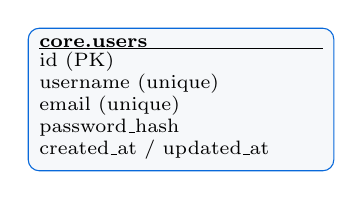
\begin{tikzpicture}[node distance=1.2cm and 2.0cm]
\node[erdent, text width=3.6cm] (users) {\textbf{core.users}\\\hrule\vspace{1pt} id (PK)\\ username (unique)\\ email (unique)\\ password\_hash\\ created\_at / updated\_at};
\end{tikzpicture}}
\caption{ERD bounded context Identity -- Bảng \texttt{core.users}}\label{fig:erd-auth}
\end{figure}


\subsubsection{Repository Catalog (siêu dữ liệu repository)}
% ====================== ERD Repository Catalog =============================
\begin{figure}[H]\centering
\resizebox{0.95\linewidth}{!}{%
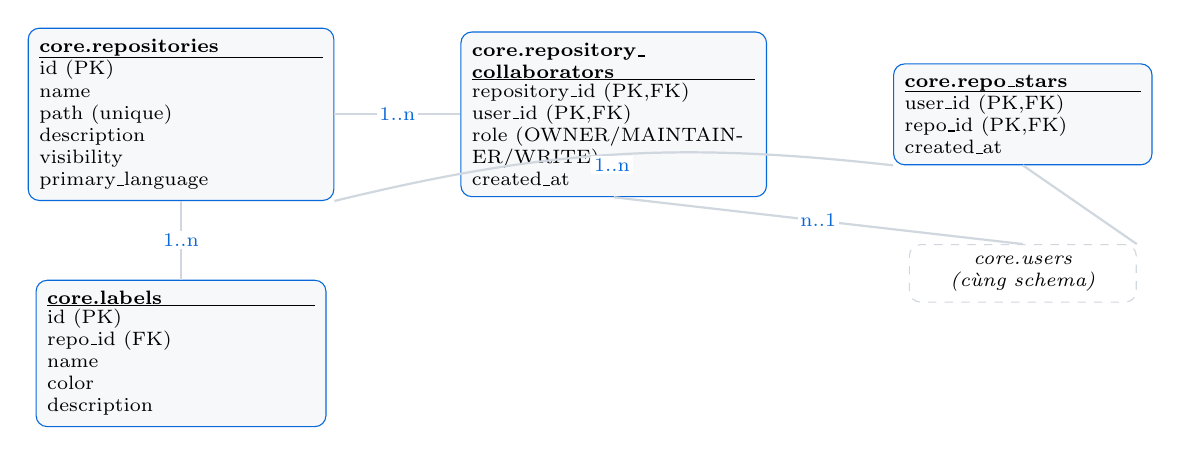
\begin{tikzpicture}[node distance=1.0cm and 1.6cm]
\node[erdent, text width=3.6cm] (repo) {\textbf{core.repositories}\\\hrule\vspace{1pt} id (PK)\\ name\\ path (unique)\\ description\\ visibility\\ primary\_language};
\node[erdent, right=of repo, text width=3.6cm] (collab) {\textbf{core.repository\_\\collaborators}\\\hrule\vspace{1pt} repository\_id (PK,FK)\\ user\_id (PK,FK)\\ role (OWNER/MAINTAINER/WRITE)\\ created\_at};
\node[erdent, right=of collab, text width=3.0cm] (star) {\textbf{core.repo\_stars}\\\hrule\vspace{1pt} user\_id (PK,FK)\\ repo\_id (PK,FK)\\ created\_at};
\node[erdent, below=of repo, text width=3.4cm] (label) {\textbf{core.labels}\\\hrule\vspace{1pt} id (PK)\\ repo\_id (FK)\\ name\\ color\\ description};
\node[erdext, below=of star] (users) {core.users\\(cùng schema)};

\draw[erdrel] (repo) -- (collab) node[erdcard,midway]{1..n};
\draw[erdrel] (repo) -- (label) node[erdcard,midway]{1..n};
\draw[erdrel] (repo.south east) to[bend left=10] node[erdcard,midway,below]{1..n} (star.south west);
\draw[erdrel] (collab.south) -- node[erdcard,midway]{n..1} (users.north);
\draw[erdrel] (star.south) -- (users.north east);
\end{tikzpicture}}
\caption{ERD bounded context Repository Catalog (\texttt{repositories}, \texttt{collaborators}, \texttt{labels}, \texttt{stars})}\label{fig:erd-repo}
\end{figure}


\subsubsection{Pull Request và sự kiện}
% ====================== ERD Pull Request ===================================
\begin{figure}[H]\centering
\resizebox{0.95\linewidth}{!}{%
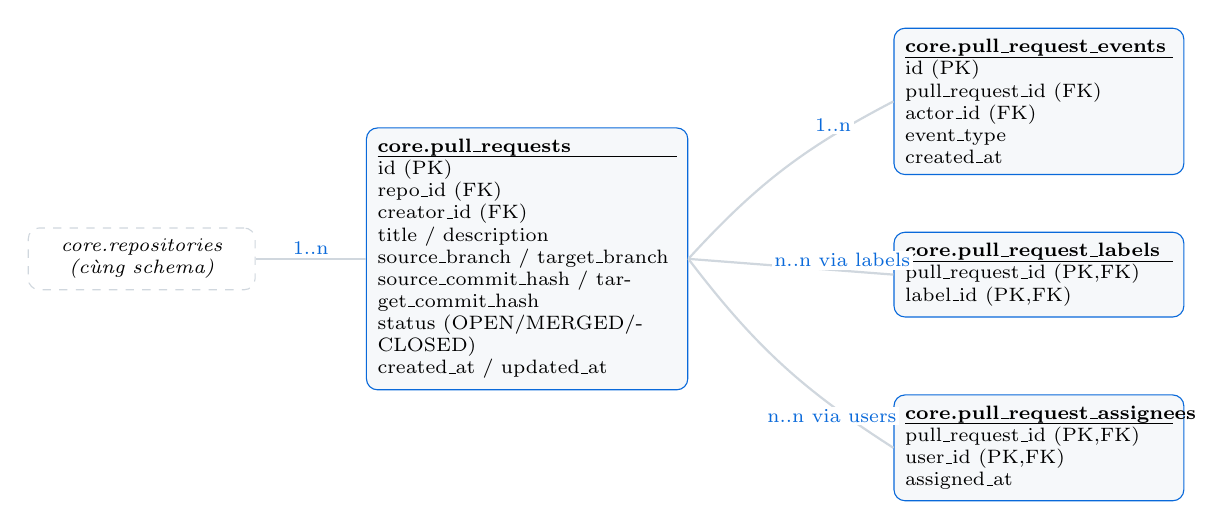
\begin{tikzpicture}
\node[erdent, text width=3.8cm] (pr) at (0,0) {\textbf{core.pull\_requests}\\\hrule\vspace{1pt} id (PK)\\ repo\_id (FK)\\ creator\_id (FK)\\ title / description\\ source\_branch / target\_branch\\ source\_commit\_hash / target\_commit\_hash\\ status (OPEN/MERGED/CLOSED)\\ created\_at / updated\_at};
\node[erdent, text width=3.4cm] (ev) at (6.5,2.0) {\textbf{core.pull\_request\_events}\\\hrule\vspace{1pt} id (PK)\\ pull\_request\_id (FK)\\ actor\_id (FK)\\ event\_type\\ created\_at};
\node[erdent, text width=3.4cm] (lbl) at (6.5,-0.2) {\textbf{core.pull\_request\_labels}\\\hrule\vspace{1pt} pull\_request\_id (PK,FK)\\ label\_id (PK,FK)};
\node[erdent, text width=3.4cm] (asn) at (6.5,-2.4) {\textbf{core.pull\_request\_assignees}\\\hrule\vspace{1pt} pull\_request\_id (PK,FK)\\ user\_id (PK,FK)\\ assigned\_at};
\node[erdext, left=1.4cm of pr] (repos) {core.repositories\\(cùng schema)};

\draw[erdrel] (pr.east) to[bend left=10] node[erdcard,near end,above]{1..n} (ev.west);
\draw[erdrel] (pr.east) -- node[erdcard,near end,above]{n..n via labels} (lbl.west);
\draw[erdrel] (pr.east) to[bend right=10] node[erdcard,near end,below]{n..n via users} (asn.west);
\draw[erdrel] (repos.east) -- node[erdcard,midway,above]{1..n} (pr.west);
\end{tikzpicture}}
\caption{ERD bounded context Pull Request (PR + sự kiện + labels + assignees)}\label{fig:erd-pr}
\end{figure}


\subsubsection{Issue, comment và sự kiện}
% ====================== ERD Issue ==========================================
\begin{figure}[H]\centering
\resizebox{0.95\linewidth}{!}{%
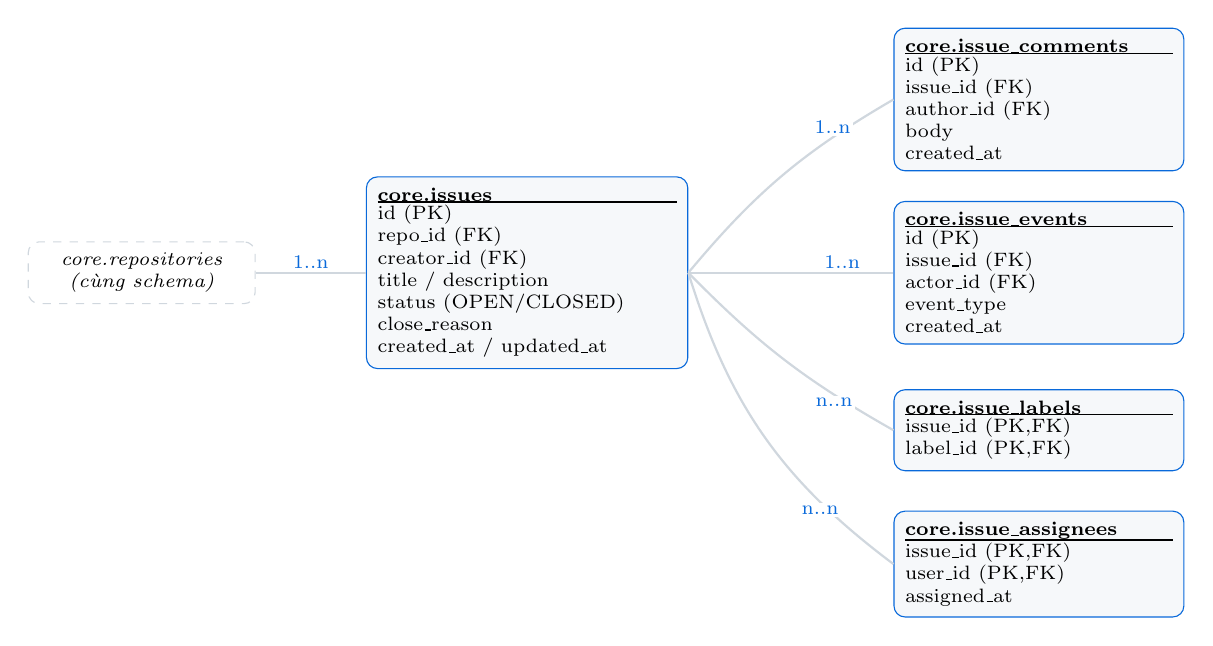
\begin{tikzpicture}
\node[erdent, text width=3.8cm] (is) at (0,0) {\textbf{core.issues}\\\hrule\vspace{1pt} id (PK)\\ repo\_id (FK)\\ creator\_id (FK)\\ title / description\\ status (OPEN/CLOSED)\\ close\_reason\\ created\_at / updated\_at};
\node[erdent, text width=3.4cm] (cm) at (6.5,2.2) {\textbf{core.issue\_comments}\\\hrule\vspace{1pt} id (PK)\\ issue\_id (FK)\\ author\_id (FK)\\ body\\ created\_at};
\node[erdent, text width=3.4cm] (ev) at (6.5,0.0) {\textbf{core.issue\_events}\\\hrule\vspace{1pt} id (PK)\\ issue\_id (FK)\\ actor\_id (FK)\\ event\_type\\ created\_at};
\node[erdent, text width=3.4cm] (lb) at (6.5,-2.0) {\textbf{core.issue\_labels}\\\hrule\vspace{1pt} issue\_id (PK,FK)\\ label\_id (PK,FK)};
\node[erdent, text width=3.4cm] (as) at (6.5,-3.7) {\textbf{core.issue\_assignees}\\\hrule\vspace{1pt} issue\_id (PK,FK)\\ user\_id (PK,FK)\\ assigned\_at};
\node[erdext, left=1.4cm of is] (repos) {core.repositories\\(cùng schema)};

\draw[erdrel] (is.east) to[bend left=10] node[erdcard,near end,above]{1..n} (cm.west);
\draw[erdrel] (is.east) -- node[erdcard,near end,above]{1..n} (ev.west);
\draw[erdrel] (is.east) to[bend right=8] node[erdcard,near end,below]{n..n} (lb.west);
\draw[erdrel] (is.east) to[bend right=18] node[erdcard,near end,below]{n..n} (as.west);
\draw[erdrel] (repos.east) -- node[erdcard,midway,above]{1..n} (is.west);
\end{tikzpicture}}
\caption{ERD bounded context Issue (issue + comments + sự kiện + labels + assignees)}\label{fig:erd-issue}
\end{figure}


\subsubsection{Insights (snapshot phân tích)}
% ====================== ERD Insights schema ================================
\begin{figure}[H]\centering
\resizebox{0.85\linewidth}{!}{%
\begin{tikzpicture}[node distance=1.0cm and 2.2cm]
\node[erdent, text width=4.0cm] (ri) {\textbf{insights.repo\_insights}\\\hrule\vspace{1pt} repo\_id (PK)\\ computed\_at\\ commits\_last\_30d\\ commit\_trend (jsonb)\\ top\_contributors (jsonb)\\ branch\_activity (jsonb)\\ primary\_language\\ language\_breakdown (jsonb)\\ last\_error};
\node[erdext, right=of ri] (cr) {core.repositories\\(schema khác,\\tham chiếu mềm)};
\draw[erdsoft] (ri) -- node[erdcard, midway, align=center]{1..1\\soft ref} (cr);
\end{tikzpicture}}
\caption{ERD schema \texttt{insights} (snapshot phân tích cho từng repository, tham chiếu mềm tới schema \texttt{core})}\label{fig:erd-insights}
\end{figure}


\subsection{Danh sách các bảng dữ liệu}
\renewcommand{\arraystretch}{1.2}
\begin{longtable}{|c|>{\ttfamily\small}p{5.0cm}|p{7.0cm}|}
\caption{Danh sách các bảng dữ liệu}\label{tab:tablelist}\\
\hline\rowcolor{sgCream}\textbf{STT} & \normalfont\textbf{Tên bảng} & \textbf{Ý nghĩa}\\\hline\endfirsthead
\hline\rowcolor{sgCream}\textbf{STT} & \normalfont\textbf{Tên bảng} & \textbf{Ý nghĩa}\\\hline\endhead
1  & core.users & Tài khoản người dùng (định danh, email, mật khẩu băm).\\\hline
2  & core.repositories & Siêu dữ liệu repository (tên, đường dẫn, mô tả, visibility, ngôn ngữ chính).\\\hline
3  & core.repository\_collaborators & Quan hệ user--repo với vai trò (OWNER/MAINTAINER/WRITE).\\\hline
4  & core.pull\_requests & Pull request với source/target branch, commit hash, trạng thái.\\\hline
5  & core.pull\_request\_events & Nhật ký sự kiện của PR (created/merged/closed/reopened/commented).\\\hline
6  & core.pull\_request\_labels & Gán label cho PR.\\\hline
7  & core.pull\_request\_assignees & Gán người phụ trách cho PR.\\\hline
8  & core.issues & Issue (title, description, status, close\_reason).\\\hline
9  & core.issue\_assignees & Gán người phụ trách cho issue.\\\hline
10 & core.issue\_events & Nhật ký sự kiện của issue.\\\hline
11 & core.issue\_comments & Bình luận trên issue.\\\hline
12 & core.issue\_labels & Gán label cho issue.\\\hline
13 & core.labels & Label (tên, màu, mô tả) thuộc về một repository.\\\hline
14 & core.repo\_stars & Quan hệ user--repo cho chức năng star.\\\hline
15 & insights.repo\_insights & Snapshot kết quả phân tích cho từng repository.\\\hline
\end{longtable}

\subsection{Thiết kế chi tiết các bảng dữ liệu}\label{sec:dbdetail}
% ====================== Đặc tả chi tiết các bảng dữ liệu =====================

\subsubsection{Bảng core.users}
\begin{dbtable}{db-users}{Chi tiết bảng core.users}
1 & id & uuid & Khoá chính (gen\_random\_uuid).\\\hline
2 & username & varchar(50) & Tên đăng nhập (duy nhất).\\\hline
3 & email & varchar(255) & Email (duy nhất).\\\hline
4 & password\_hash & varchar(255) & Mật khẩu băm bằng bcrypt.\\\hline
5 & created\_at & timestamptz & Thời điểm đăng ký.\\\hline
6 & updated\_at & timestamptz & Thời điểm cập nhật gần nhất (vd. đổi username).\\\hline
\end{dbtable}

\subsubsection{Bảng core.repositories}
\begin{dbtable}{db-repos}{Chi tiết bảng core.repositories}
1 & id & uuid & Khoá chính.\\\hline
2 & name & varchar(255) & Tên repository.\\\hline
3 & path & varchar(1024) & Đường dẫn tương đối tới thư mục repo trên hệ thống tệp, dạng \texttt{<owner>/<name>.git} (duy nhất).\\\hline
4 & created\_at & timestamptz & Thời điểm tạo.\\\hline
5 & description & text & Mô tả repo.\\\hline
6 & visibility & varchar(16) & PUBLIC / PRIVATE.\\\hline
7 & primary\_language & varchar(64) & Ngôn ngữ chính (cập nhật bởi Insights).\\\hline
\end{dbtable}

\subsubsection{Bảng core.repository\_collaborators}
\begin{dbtable}{db-collab}{Chi tiết bảng core.repository\_collaborators}
1 & repository\_id & uuid & Khoá chính (kết hợp), FK $\to$ \texttt{core.repositories(id)} ON DELETE CASCADE.\\\hline
2 & user\_id & uuid & Khoá chính (kết hợp), FK $\to$ \texttt{core.users(id)} ON DELETE CASCADE.\\\hline
3 & role & varchar(20) & Vai trò: OWNER / MAINTAINER / WRITE.\\\hline
4 & created\_at & timestamptz & Thời điểm thêm collaborator.\\\hline
\end{dbtable}

\subsubsection{Bảng core.pull\_requests}
\begin{dbtable}{db-pulls}{Chi tiết bảng core.pull\_requests}
1 & id & uuid & Khoá chính.\\\hline
2 & repo\_id & uuid & FK $\to$ \texttt{core.repositories(id)} ON DELETE CASCADE.\\\hline
3 & creator\_id & uuid & FK $\to$ \texttt{core.users(id)}.\\\hline
4 & title & varchar(255) & Tiêu đề PR.\\\hline
5 & description & text & Mô tả PR (Markdown).\\\hline
6 & source\_branch & varchar(255) & Branch nguồn (head).\\\hline
7 & target\_branch & varchar(255) & Branch đích (base).\\\hline
8 & source\_commit\_hash & varchar(64) & SHA-1 commit head ở thời điểm tạo PR.\\\hline
9 & target\_commit\_hash & varchar(64) & SHA-1 commit base ở thời điểm tạo PR.\\\hline
10 & status & varchar(16) & OPEN / MERGED / CLOSED.\\\hline
11 & created\_at & timestamptz & Thời điểm tạo PR.\\\hline
12 & updated\_at & timestamptz & Thời điểm cập nhật trạng thái cuối.\\\hline
\end{dbtable}

\subsubsection{Bảng core.pull\_request\_events}
\begin{dbtable}{db-prevents}{Chi tiết bảng core.pull\_request\_events}
1 & id & uuid & Khoá chính.\\\hline
2 & pull\_request\_id & uuid & FK $\to$ \texttt{core.pull\_requests(id)} ON DELETE CASCADE.\\\hline
3 & actor\_id & uuid & FK $\to$ \texttt{core.users(id)}.\\\hline
4 & event\_type & varchar(32) & Loại sự kiện: created / merged / closed / reopened / commented \ldots\\\hline
5 & created\_at & timestamptz & Thời điểm sự kiện.\\\hline
\end{dbtable}

\subsubsection{Bảng core.pull\_request\_labels}
\begin{dbtable}{db-prlabel}{Chi tiết bảng core.pull\_request\_labels}
1 & pull\_request\_id & uuid & Khoá chính (kết hợp), FK $\to$ \texttt{core.pull\_requests(id)} ON DELETE CASCADE.\\\hline
2 & label\_id & uuid & Khoá chính (kết hợp), FK $\to$ \texttt{core.labels(id)} ON DELETE CASCADE.\\\hline
\end{dbtable}

\subsubsection{Bảng core.pull\_request\_assignees}
\begin{dbtable}{db-prassign}{Chi tiết bảng core.pull\_request\_assignees}
1 & pull\_request\_id & uuid & Khoá chính (kết hợp), FK $\to$ \texttt{core.pull\_requests(id)} ON DELETE CASCADE.\\\hline
2 & user\_id & uuid & Khoá chính (kết hợp), FK $\to$ \texttt{core.users(id)} ON DELETE CASCADE.\\\hline
3 & assigned\_at & timestamptz & Thời điểm gán.\\\hline
\end{dbtable}

\subsubsection{Bảng core.issues}
\begin{dbtable}{db-issues}{Chi tiết bảng core.issues}
1 & id & uuid & Khoá chính.\\\hline
2 & repo\_id & uuid & FK $\to$ \texttt{core.repositories(id)} ON DELETE CASCADE.\\\hline
3 & creator\_id & uuid & FK $\to$ \texttt{core.users(id)}.\\\hline
4 & title & text & Tiêu đề issue.\\\hline
5 & description & text & Mô tả issue (Markdown).\\\hline
6 & status & varchar(16) & OPEN / CLOSED.\\\hline
7 & close\_reason & varchar(24) & COMPLETED / NOT\_PLANNED / DUPLICATE (NULL nếu OPEN).\\\hline
8 & created\_at & timestamptz & Thời điểm tạo.\\\hline
9 & updated\_at & timestamptz & Thời điểm cập nhật trạng thái cuối.\\\hline
\end{dbtable}

\subsubsection{Bảng core.issue\_assignees}
\begin{dbtable}{db-issueassign}{Chi tiết bảng core.issue\_assignees}
1 & issue\_id & uuid & Khoá chính (kết hợp), FK $\to$ \texttt{core.issues(id)} ON DELETE CASCADE.\\\hline
2 & user\_id & uuid & Khoá chính (kết hợp), FK $\to$ \texttt{core.users(id)} ON DELETE CASCADE.\\\hline
3 & assigned\_at & timestamptz & Thời điểm gán.\\\hline
\end{dbtable}

\subsubsection{Bảng core.issue\_events}
\begin{dbtable}{db-issueevents}{Chi tiết bảng core.issue\_events}
1 & id & uuid & Khoá chính.\\\hline
2 & issue\_id & uuid & FK $\to$ \texttt{core.issues(id)} ON DELETE CASCADE.\\\hline
3 & actor\_id & uuid & FK $\to$ \texttt{core.users(id)}.\\\hline
4 & event\_type & varchar(32) & Loại sự kiện: created / closed / reopened / commented / labeled / assigned \ldots\\\hline
5 & created\_at & timestamptz & Thời điểm sự kiện.\\\hline
\end{dbtable}

\subsubsection{Bảng core.issue\_comments}
\begin{dbtable}{db-issuecmt}{Chi tiết bảng core.issue\_comments}
1 & id & uuid & Khoá chính.\\\hline
2 & issue\_id & uuid & FK $\to$ \texttt{core.issues(id)} ON DELETE CASCADE.\\\hline
3 & author\_id & uuid & FK $\to$ \texttt{core.users(id)}.\\\hline
4 & body & text & Nội dung comment (Markdown).\\\hline
5 & created\_at & timestamptz & Thời điểm comment.\\\hline
\end{dbtable}

\subsubsection{Bảng core.issue\_labels}
\begin{dbtable}{db-issuelabel}{Chi tiết bảng core.issue\_labels}
1 & issue\_id & uuid & Khoá chính (kết hợp), FK $\to$ \texttt{core.issues(id)} ON DELETE CASCADE.\\\hline
2 & label\_id & uuid & Khoá chính (kết hợp), FK $\to$ \texttt{core.labels(id)} ON DELETE CASCADE.\\\hline
\end{dbtable}

\subsubsection{Bảng core.labels}
\begin{dbtable}{db-labels}{Chi tiết bảng core.labels}
1 & id & uuid & Khoá chính.\\\hline
2 & repo\_id & uuid & FK $\to$ \texttt{core.repositories(id)} ON DELETE CASCADE.\\\hline
3 & name & varchar(50) & Tên label (duy nhất trong cùng repo).\\\hline
4 & color & varchar(7) & Mã màu HEX, ví dụ \texttt{\#d73a4a}.\\\hline
5 & description & text & Mô tả label.\\\hline
6 & created\_at & timestamptz & Thời điểm tạo.\\\hline
\end{dbtable}

\subsubsection{Bảng core.repo\_stars}
\begin{dbtable}{db-stars}{Chi tiết bảng core.repo\_stars}
1 & user\_id & uuid & Khoá chính (kết hợp), FK $\to$ \texttt{core.users(id)} ON DELETE CASCADE.\\\hline
2 & repo\_id & uuid & Khoá chính (kết hợp), FK $\to$ \texttt{core.repositories(id)} ON DELETE CASCADE.\\\hline
3 & created\_at & timestamptz & Thời điểm star.\\\hline
\end{dbtable}

\subsubsection{Bảng insights.repo\_insights}
\begin{dbtable}{db-insights}{Chi tiết bảng insights.repo\_insights}
1 & repo\_id & uuid & Khoá chính, tham chiếu mềm tới \texttt{core.repositories(id)}.\\\hline
2 & computed\_at & timestamptz & Thời điểm tính toán snapshot.\\\hline
3 & commits\_last\_30d & int & Số commit trong 30 ngày gần nhất.\\\hline
4 & commit\_trend & jsonb & Mảng \texttt{[\{date, commit\_count\}]} group theo ngày.\\\hline
5 & top\_contributors & jsonb & Mảng \texttt{[\{author\_name, commit\_count\}]} top theo số commit.\\\hline
6 & branch\_activity & jsonb & Mảng \texttt{[\{branch\_name, commit\_count\}]}.\\\hline
7 & primary\_language & varchar(64) & Ngôn ngữ chiếm tỉ lệ cao nhất.\\\hline
8 & language\_breakdown & jsonb & Mảng \texttt{[\{language, bytes, percentage\}]}.\\\hline
9 & last\_error & text & Thông báo lỗi của lần tính cuối (NULL nếu thành công).\\\hline
\end{dbtable}


\section{Thiết kế nghiệp vụ đặc thù}

\subsection{Giao thức Git Smart HTTP}
Synergit hiện thực đầy đủ ba endpoint của Git Smart HTTP ở dịch vụ GitStorage để hỗ trợ \texttt{git clone/push/pull/fetch}:

\begin{itemize}
\item \texttt{GET /:username/:repo.git/info/refs?service=<service>} -- advertise refs.
\item \texttt{POST /:username/:repo.git/git-upload-pack} -- gửi packfile cho client (clone/fetch).
\item \texttt{POST /:username/:repo.git/git-receive-pack} -- nhận packfile từ client (push).
\end{itemize}

Cả ba endpoint được Gateway forward thẳng tới GitStorage. Không yêu cầu xác thực JWT đối với repository PUBLIC; với repository PRIVATE, GitStorage trả về \texttt{401 Unauthorized}.

\subsection{Đảm bảo nhất quán khi đổi username}
Khi người dùng đổi username, có ba thay đổi phải xảy ra cùng lúc:

\begin{enumerate}
\item Cập nhật trường \texttt{username} trong \texttt{core.users}.
\item Đổi tên thư mục \texttt{D:\textbackslash SynergitRepo\textbackslash<old\_username>\textbackslash} $\to$ \texttt{D:\textbackslash SynergitRepo\textbackslash<new\_username>\textbackslash}.
\item Cập nhật cột \texttt{path} trong \texttt{core.repositories} cho mọi repo của user (thay tiền tố \texttt{<old>/} bằng \texttt{<new>/}).
\item Phát hành JWT mới chứa username mới (vì JWT cũ vẫn ghi username cũ).
\end{enumerate}

Dịch vụ Core thực hiện toàn bộ các bước trên trong cùng một handler: cập nhật DB, gọi GitStorage qua HTTP để đổi tên thư mục, cập nhật \texttt{repositories.path}, phát hành JWT mới và trả về client. Frontend nhận JWT mới, lưu vào \texttt{localStorage} và reload trang.

\subsection{Máy trạng thái Pull Request}
Mỗi pull request tuân theo một máy trạng thái (FSM); mọi chuyển trạng thái đều được ghi vào bảng \texttt{core.pull\_request\_events} kèm thời điểm và người thực hiện. Sơ đồ FSM được trình bày trong Hình~\ref{fig:pr-fsm}.

% ====================== Máy trạng thái Pull Request (TikZ) =================
\begin{figure}[H]
\centering
\resizebox{0.92\linewidth}{!}{%
\begin{tikzpicture}[
  font=\sffamily\small, node distance=2.0cm,
  st/.style={draw=sgBlue, fill=sgCream, rounded corners, minimum height=0.95cm,
             minimum width=2.4cm, align=center, font=\sffamily\footnotesize},
  term/.style={st, fill=green!12, draw=sgAccent},
  cancel/.style={st, fill=red!10, draw=red!60},
  arr/.style={-{Latex[length=2mm]}, draw=sgBlue, thick, font=\sffamily\scriptsize},
]
\node[st] (open) {OPEN\\\scriptsize đang mở};
\node[term, right=of open] (merged) {MERGED\\\scriptsize đã merge};
\node[cancel, below=1.4cm of merged] (closed) {CLOSED\\\scriptsize đã đóng};

\draw[arr] (open) -- node[above, midway]{merge} (merged);
\draw[arr] (open) to[bend right=15] node[below, near start]{close} (closed);
\draw[arr] (closed) to[bend right=15] node[above, near end]{reopen} (open);
\draw[arr] (merged) -- node[right, midway]{revert (tạo PR mới)} (closed);
\end{tikzpicture}}
\caption{Máy trạng thái (FSM) vòng đời Pull Request}
\label{fig:pr-fsm}
\end{figure}

\begin{figure}[H]
\centering
\resizebox{0.7\linewidth}{!}{%
\begin{tikzpicture}[
  font=\sffamily\small, node distance=2.0cm,
  st/.style={draw=sgBlue, fill=sgCream, rounded corners, minimum height=0.95cm,
             minimum width=2.4cm, align=center, font=\sffamily\footnotesize},
  cancel/.style={st, fill=red!10, draw=red!60},
  arr/.style={-{Latex[length=2mm]}, draw=sgBlue, thick, font=\sffamily\scriptsize},
]
\node[st] (open) {OPEN\\\scriptsize đang mở};
\node[cancel, right=of open] (closed) {CLOSED\\\scriptsize đã đóng};

\draw[arr] (open) to[bend left=15] node[above, midway]{close (lý do)} (closed);
\draw[arr] (closed) to[bend left=15] node[below, midway]{reopen} (open);
\end{tikzpicture}}
\caption{Máy trạng thái (FSM) vòng đời Issue (lý do đóng: COMPLETED / NOT\_PLANNED / DUPLICATE)}
\label{fig:issue-fsm}
\end{figure}


\subsection{Cơ chế giải quyết xung đột merge}
Khi merge một pull request, dịch vụ Core gọi \texttt{CompareRefs} qua GitStorage để kiểm tra khả năng merge. Nếu \texttt{Mergeable = false}:

\begin{enumerate}
\item Frontend chuyển sang giao diện ``Resolve conflicts'' và gọi \texttt{GET /api/v1/repos/:repo\_id/pulls/:pull\_id/conflicts}.
\item Core gọi GitStorage \texttt{GetConflictingFiles} để lấy danh sách file xung đột; với mỗi file, gọi \texttt{GetConflictContent} để lấy nội dung file đã chèn marker (\texttt{<<<<<<<}, \texttt{=======}, \texttt{>>>>>>>}).
\item Người dùng chỉnh sửa nội dung trên trình soạn thảo trong giao diện web để giải quyết xung đột.
\item Frontend gửi danh sách \texttt{ConflictResolution\{Path, ResolvedContent\}} qua \texttt{POST /api/v1/repos/:repo\_id/pulls/:pull\_id/conflicts/resolve}.
\item Core gọi GitStorage \texttt{ResolveConflictsAndCommit}; GitStorage commit nội dung đã giải quyết lên source branch của PR và push.
\item PR có thể merge ở lần thử tiếp theo.
\end{enumerate}

\subsection{Tính toán Insights theo yêu cầu}
Insights được tính theo phương thức ``recompute on demand'': khi người dùng vào trang Insights của một repo, frontend gọi \texttt{GET /api/v1/repos/:id/insights} để lấy snapshot mới nhất từ \texttt{insights.repo\_insights}. Người dùng có nút ``Recompute'' để chủ động tính lại; khi đó frontend gọi \texttt{POST /api/v1/repos/:id/insights/recompute}, dịch vụ Insights:

\begin{enumerate}
\item Lấy danh sách commit của tất cả branch (qua GitStorage HTTP).
\item Lấy thông tin từng branch (last commit, ahead/behind).
\item Tính \textit{commits\_last\_30d}, \textit{commit\_trend} (group by ngày), \textit{top\_contributors} (group by author).
\item Tính \textit{branch\_activity} (số commit mỗi branch).
\item Gọi GitStorage \texttt{GetLanguageBreakdown} để lấy phân bố ngôn ngữ (theo \% byte).
\item Lưu kết quả vào \texttt{insights.repo\_insights} (upsert theo \texttt{repo\_id}).
\end{enumerate}

Profile Activity tương tự nhưng tổng hợp dữ liệu commit của tất cả repo mà người dùng có quyền, kết hợp với số lượng issue và PR đã tạo từ \texttt{core.*}.

\chapter{Xây dựng website}

Chương 4 trình bày quá trình xây dựng giao diện và hiện thực hoá các chức năng của hệ thống Synergit, từ việc thiết kế template giao diện (layout, hệ màu, font chữ, bộ thành phần dùng chung) đến việc áp dụng template để xây dựng các trang chính: đăng nhập, dashboard repository, code browser, pull request, issue, profile và settings. Chương cũng minh hoạ một số đoạn mã tiêu biểu ở cả frontend và backend.

\section{Thiết kế Template}

\subsection{Phác thảo layout website}
Giao diện Synergit lấy cảm hứng trực tiếp từ GitHub để giảm chi phí học của người dùng. Toàn bộ ứng dụng dùng layout dạng \textit{TopHeader} (thanh điều hướng dọc trên cùng) + \textit{nội dung chính} dạng tab, không có sidebar trái -- y hệt GitHub. Các trang con bên trong một repository chia thành 4 tab cố định: \textbf{Code}, \textbf{Pull Requests}, \textbf{Issues}, \textbf{Insights}.

\subsection{Hệ màu và nhận diện thương hiệu}
Synergit dùng bảng màu lấy cảm hứng từ GitHub: tông \textbf{xanh lam} \texttt{\#0969DA} (\texttt{sgBlue}) làm màu nhấn chủ đạo, kết hợp nền nhạt \texttt{\#F6F8FA} (\texttt{sgCream}), chữ màu mực \texttt{\#1F2328} (\texttt{sgInk}) và đường kẻ phân chia \texttt{\#D0D7DE} (\texttt{sgLine}). Màu phụ \texttt{\#2DA44E} (\texttt{sgAccent}) được dùng cho trạng thái thành công (PR đã merged). Hệ màu được định nghĩa thành các \textit{CSS variables} trong Tailwind, cho phép chuyển sang giao diện tối trong tương lai.

\subsection{Font chữ và iconography}
Hệ thống sử dụng font sans-serif hệ thống (\texttt{system-ui}) cho phần lớn giao diện và font \texttt{ui-monospace} cho code/diff. Bộ icon kết hợp:
\begin{itemize}
\item \textbf{Lucide:} cho các thao tác chung (settings, search, x, plus\ldots).
\item \textbf{Octicons (do GitHub thiết kế):} cho các icon đặc trưng của hệ thống quản lý mã nguồn -- \textit{git-branch}, \textit{git-commit}, \textit{git-pull-request}, \textit{git-pull-request-closed}, \textit{git-merge}, \textit{git-compare}, \textit{repo}, \textit{issue-opened}, \textit{issue-closed}, \textit{star}\ldots
\end{itemize}

Các Octicon được vẽ thuần SVG ngay trong file \texttt{components/icons/Octicons.tsx} để bảo đảm hiển thị sắc nét và không phụ thuộc thư viện ngoài.

\section{Áp dụng Template xây dựng các trang web}

\subsection{Trang đăng nhập và đăng ký}
Trang đăng nhập là điểm vào của ứng dụng. Người dùng nhập tên đăng nhập (hoặc email) và mật khẩu; nếu hợp lệ, hệ thống cấp JWT và chuyển tới dashboard. Trang đăng ký tương tự, yêu cầu thêm email và mật khẩu tối thiểu 6 ký tự.

\figauto{image/synergit-dang-nhap.png}{Giao diện trang đăng nhập}{7cm}
\figauto{image/synergit-dang-ky.png}{Giao diện trang đăng ký tài khoản}{7cm}

\subsection{Trang dashboard repository (Home)}
Sau khi đăng nhập, người dùng vào dashboard hiển thị danh sách các repository sở hữu/cộng tác, kèm các thẻ thống kê (số repo, số star, số PR). Trang có nút ``New repository'' nổi bật để tạo nhanh.

\figauto{image/synergit-dashboard.png}{Giao diện Dashboard liệt kê repository}{6.5cm}

\subsection{Trang tạo repository}
Trang tạo repo cho phép nhập tên, mô tả, chọn visibility (PUBLIC/PRIVATE), bật/tắt khởi tạo file \texttt{README.md}, chọn template \texttt{.gitignore} và \texttt{LICENSE}. Sau khi tạo, người dùng được chuyển tới trang Code của repo mới.

\figauto{image/synergit-tao-repo.png}{Giao diện tạo repository mới}{6.5cm}

\subsection{Trang Code -- Code browser}
Trang Code là trung tâm nghiệp vụ của một repository. Trang này hiển thị: thanh điều hướng repo (Code/PR/Issues/Insights), thanh chọn branch (\texttt{BranchTagMenu}), nút điều hướng nhánh (Branches), file explorer dạng tree, và phần xem nội dung file (kèm tô màu cú pháp). Khi mở một file, panel commit history hiển thị lịch sử commit của file đó.

\figauto{image/synergit-code-browser.png}{Giao diện trang Code -- File explorer + Commit history}{8cm}
\figauto{image/synergit-file-content.png}{Giao diện xem nội dung file kèm syntax highlight}{6.5cm}

Đoạn mã sau minh hoạ cách frontend gọi API để lấy cây thư mục:

\begin{lstlisting}[language=TypeScript, caption={Lấy cây thư mục của repo theo branch (frontend)}]
// services/api/repos.ts (rút gọn)
export const reposApi = {
  getTree: (repoId: string, path = '', branch = '') =>
    fetcher<RepoFile[]>(
      `/repos/${repoId}/tree?path=${encodeURIComponent(path)}&branch=${encodeURIComponent(branch)}`,
    ),

  getBlob: (repoId: string, path: string, branch = '') =>
    fetcher<{ content: string } | string>(
      `/repos/${repoId}/blob?path=${encodeURIComponent(path)}&branch=${encodeURIComponent(branch)}`,
    ),

  getCommits: (repoId: string, branch = '', path = '') => {
    const params = new URLSearchParams();
    params.set('branch', branch);
    if (path.trim()) params.set('path', path);
    return fetcher<Commit[]>(`/repos/${repoId}/commits?${params.toString()}`);
  },
};
\end{lstlisting}

Phía backend (dịch vụ Core), handler nhận request và uỷ quyền cho usecase rồi gọi GitStorage qua HTTP client adapter:

\begin{lstlisting}[language=Go, caption={Handler lấy tree (Core service, rút gọn)}]
// HandleGetTree kiểm tra quyền truy cập repo, gọi usecase, trả JSON.
func (h *RepoHandler) HandleGetTree(c *gin.Context) {
    requesterID, _ := parseRequesterID(c)
    repoID := uuid.MustParse(c.Param("repo_id"))
    branch := c.Query("branch")
    path := c.Query("path")

    files, err := h.repoUseCase.GetTree(c, requesterID, repoID, path, branch)
    if err != nil { response.Error(c, err); return }
    c.JSON(http.StatusOK, files)
}
\end{lstlisting}

\subsection{Trang Branches}
Trang Branches liệt kê toàn bộ branch của repository, cho mỗi branch hiển thị: tên, người commit gần nhất, thời điểm cập nhật, số commit ahead/behind so với branch mặc định. Người dùng có thể tạo branch mới (từ branch nào tuỳ chọn), đổi tên, xoá branch.

\figauto{image/synergit-branches.png}{Giao diện trang Branches}{6.5cm}

\subsection{Trang Commits và chi tiết Commit}
Trang Commit history liệt kê các commit theo branch hiện tại; mỗi commit hiển thị: avatar tác giả (chữ cái đầu), tên, message, hash rút gọn (kèm nút copy), thời gian. Nhấp vào hash mở trang chi tiết commit với diff theo từng file (unified diff).

\figauto{image/synergit-commits.png}{Giao diện danh sách commit}{6cm}
\figauto{image/synergit-commit-diff.png}{Giao diện chi tiết commit kèm diff theo file}{8cm}

\subsection{Trang Pull Requests}
Trang \textbf{Pull Requests Board} liệt kê các PR theo bộ lọc trạng thái (Open/Closed); mỗi PR hiển thị: title (kèm icon trạng thái), số PR, branch source $\to$ target, label, assignee (avatar), comment count. Bộ lọc đa lựa chọn cho author, label, assignee.

\figauto{image/synergit-pr-board.png}{Giao diện danh sách Pull Request (Board)}{7.5cm}

\subsubsection{Tạo Pull Request: trang Compare}
Trước khi tạo PR, người dùng chọn base/head trên trang Compare; hệ thống hiển thị các commit khác biệt và các file thay đổi. Nếu base = head, hiện thông báo ``There isn't anything to compare''.

\figauto{image/synergit-compare.png}{Giao diện so sánh hai branch (Compare)}{7cm}

\subsubsection{Chi tiết Pull Request}
Trang chi tiết PR có 4 phần: tiêu đề + trạng thái, dòng thời gian sự kiện (event timeline), tab Conversation/Commits/Files changed, panel Merge bên dưới. Khi PR ở trạng thái OPEN, panel Merge cho phép chọn commit message (mặc định theo format GitHub), nhấn ``Merge pull request''. Khi đã merged, panel hiện nút ``Revert''.

\figauto{image/synergit-pr-detail.png}{Giao diện chi tiết Pull Request kèm event timeline}{8cm}
\figauto{image/synergit-pr-merge.png}{Giao diện panel Merge với commit message tuỳ chỉnh}{6cm}

Đoạn mã sau minh hoạ luồng merge phía backend (Core service):

\begin{lstlisting}[language=Go, caption={Usecase merge pull request (Core service)}]
// MergePullRequest: kiểm tra quyền, gọi GitStorage để merge, cập nhật trạng thái.
func (s *PullRequestService) MergePullRequest(
    ctx context.Context, requesterID, repoID, pullID uuid.UUID,
    commitMessage, commitDescription string,
) error {
    pr, err := s.prStore.GetByID(pullID)
    if err != nil { return err }
    if pr.Status != domain.PullRequestStatusOpen {
        return errors.New("pull request is not open")
    }

    role, _ := s.collabStore.GetRole(repoID, requesterID)
    if !role.CanManageCollaborators() { // OWNER hoặc MAINTAINER
        return errors.New("permission denied")
    }

    repo, _ := s.repoStore.GetByID(repoID)
    merger, _ := s.userStore.GetUserByID(requesterID)

    // Gọi GitStorage qua port.GitManager (HTTP client trong môi trường multi-service).
    if err := s.gitManager.MergeBranches(
        repo.Path, pr.SourceBranch, pr.TargetBranch,
        merger.Username, buildMessage(commitMessage, commitDescription),
    ); err != nil {
        return err
    }

    // Cập nhật trạng thái PR và ghi sự kiện.
    pr.Status = domain.PullRequestStatusMerged
    s.prStore.Update(pr)
    s.prStore.AddEvent(pullID, requesterID, "merged")
    return nil
}
\end{lstlisting}

\subsubsection{Resolve conflicts}
Khi merge gặp conflict, frontend chuyển sang trang Resolve. Mỗi file conflict hiển thị nội dung kèm marker chuẩn của Git (\texttt{<<<<<<<}, \texttt{=======}, \texttt{>>>>>>>}); người dùng chỉnh sửa trong trình soạn thảo và nhấn ``Mark as resolved''. Sau khi tất cả file được resolve, nhấn ``Commit merge'' để gửi nội dung đã giải quyết về backend.

\figauto{image/synergit-resolve.png}{Giao diện resolve conflict}{7cm}

\subsection{Trang Issues}
Trang \textbf{Issue Board} cũng có cấu trúc tương tự PR: bộ lọc trạng thái Open/Closed, lọc theo author/label/assignee. Trang chi tiết issue cho phép comment (Markdown), gán/bỏ assignee, gán/bỏ label, đóng kèm lý do (COMPLETED/NOT\_PLANNED/DUPLICATE) hoặc mở lại.

\figauto{image/synergit-issue-board.png}{Giao diện danh sách Issue (Board)}{7cm}
\figauto{image/synergit-issue-detail.png}{Giao diện chi tiết Issue với comment và timeline}{7.5cm}

\subsection{Trang Insights -- Repo Insights}
Trang Repo Insights hiển thị các bảng phân tích cho repository: commit trend 30 ngày (line chart), top contributors (bảng), branch activity (bảng), language breakdown (biểu đồ tròn). Nút ``Recompute'' ở góc phải kích hoạt tính lại snapshot.

\figauto{image/synergit-repo-insights.png}{Giao diện Repo Insights}{7.5cm}

\subsection{Trang Profile -- Contribution Graph}
Trang Profile hiển thị thông tin người dùng (avatar, username, bio) cùng \textbf{Contribution Graph} kiểu GitHub -- một heatmap 7 hàng x ~53 cột thể hiện số commit mỗi ngày trong 365 ngày qua. Bên dưới là Activity Overview (số commit, code review, issue, PR; top repository đóng góp).

\figauto{image/synergit-profile-overview.png}{Giao diện Profile kèm Contribution Graph 365 ngày}{8cm}
\figauto{image/synergit-profile-repos.png}{Giao diện Profile -- Tab Repositories}{6.5cm}

Đoạn mã sau minh hoạ cách dịch vụ Insights tổng hợp dữ liệu Profile Activity:

\begin{lstlisting}[language=Go, caption={Tổng hợp Profile Activity (Insights service, rút gọn)}]
// GetProfileActivity tính toán contribution graph 365 ngày + activity overview.
func (s *RepoInsightsService) GetProfileActivity(
    requesterID uuid.UUID, year int,
) (*domain.ProfileActivitySnapshot, error) {
    user, _ := s.userStore.GetUserByID(requesterID)
    repos, _ := s.repoStore.ListRepositoriesForUser(requesterID)

    // Đếm contribution theo ngày bằng cách quét commits của tất cả repo.
    activity, err := s.metricComputer.ComputeProfileCommitActivity(
        ctx, repos, user.Username, year, time.Now(),
    )
    if err != nil { return nil, err }

    // Đếm số issue & PR đã tạo (đọc qua adapter sang core schema).
    issues := s.issueStore.CountByCreatorAndYear(requesterID, year)
    prs := s.prStore.CountByCreatorAndYear(requesterID, year)

    return &domain.ProfileActivitySnapshot{
        Username: user.Username, SelectedYear: year,
        ContributionDays: activity.ContributionDays,
        TotalContributions: activity.TotalContributions,
        ActivityChart: domain.ProfileActivityChart{
            Commits: activity.TotalContributions,
            Issues: issues, PullRequests: prs,
        },
        ActivityOverview: domain.ProfileActivityOverview{
            TopRepositories: activity.TopRepositories,
            OtherRepoCount: activity.OtherRepoCount,
            CommitsLast365Days: activity.CommitsLast365Days,
        },
    }, nil
}
\end{lstlisting}

\subsection{Trang Settings -- Account}
Trang Settings/Account cho phép người dùng đổi tên đăng nhập (đổi cả thư mục lưu repo, đường dẫn trong DB và phát hành JWT mới), đăng xuất khỏi tất cả thiết bị (vô hiệu hoá JWT cũ).

\figauto{image/synergit-settings.png}{Giao diện trang Settings -- Account (đổi username)}{6.5cm}

\subsection{API Gateway và phân tách dịch vụ}
Toàn bộ frontend chỉ giao tiếp với một URL duy nhất (\texttt{http://localhost:8080}) -- chính là Gateway. Gateway dùng \texttt{net/http/httputil.ReverseProxy} để định tuyến request:

\begin{lstlisting}[language=Go, caption={Định tuyến của Gateway theo prefix đường dẫn}]
// internal/proxy/router.go (rút gọn)
type Rule struct {
    Prefix   string
    Upstream *url.URL
}

func BuildRules(env Env) []Rule {
    return []Rule{
        {Prefix: "/api/v1/insights", Upstream: env.InsightsURL},
        {Prefix: "/api/v1/profile/activity", Upstream: env.InsightsURL},
        {Prefix: "/api/v1/git", Upstream: env.GitStorageURL},
        // Mặc định: tất cả request không khớp prefix nào ở trên -> Core.
        {Prefix: "/", Upstream: env.CoreURL},
    }
}

func (rt *Router) ServeHTTP(w http.ResponseWriter, r *http.Request) {
    for _, rule := range rt.rules {
        if strings.HasPrefix(r.URL.Path, rule.Prefix) {
            httputil.NewSingleHostReverseProxy(rule.Upstream).ServeHTTP(w, r)
            return
        }
    }
}
\end{lstlisting}

Với cách định tuyến này, frontend không cần biết về số lượng và vị trí của các dịch vụ backend: thêm/bớt dịch vụ chỉ là việc thêm/bớt rule trong Gateway và biến môi trường.

\chapter{Kết luận}

Sau quá trình nghiên cứu, thiết kế và triển khai thực nghiệm, đề tài \textit{``Synergit -- Ứng dụng quản lý quy trình phát triển phần mềm tích hợp quản lý mã nguồn dự án áp dụng kiến trúc Microservices''} đã hoàn thành các mục tiêu đặt ra. Dự án không chỉ là một ``GitHub thu nhỏ'' về mặt tính năng (đăng ký, repository, push/pull/clone, code browser, pull request, issue, label, collaborator, star, insights, profile activity), mà còn là một mô hình tham khảo cho việc áp dụng \textit{Domain-Driven Design (DDD)} và \textit{Clean Architecture} để xây dựng một hệ thống Microservices thực dụng theo triết lý ``Majestic Monolith + Strategic Services'' của GitHub. Việc kết hợp Go + Gin ở backend, React + TypeScript + Vite ở frontend, PostgreSQL với schema-per-service và go-git ở dịch vụ GitStorage đã tạo nên một nền tảng vững chắc, đáp ứng nhu cầu của một đội phát triển nội bộ vừa và nhỏ muốn tự triển khai (self-hosted) hệ thống quản lý mã nguồn của riêng mình.

\section{Ưu điểm của đồ án}
\begin{itemize}
\item \textbf{Tính năng cộng tác đầy đủ kiểu GitHub:} Hệ thống cung cấp toàn bộ vòng đời phát triển: tạo repository, push/clone/pull qua Git Smart HTTP, duyệt mã nguồn với syntax highlight, commit qua web, quản lý branch (kèm thông tin ahead/behind), so sánh branch (compare), pull request với event timeline, merge và revert, phát hiện và giải quyết xung đột (merge conflict) qua giao diện web, issue tracking với label/assignee/comment và lý do đóng (completed/not\_planned/duplicate), star repository, contribution graph 365 ngày kiểu GitHub.
\item \textbf{Kiến trúc Microservices thực dụng theo triết lý GitHub:} Hệ thống được tách thành 4 binary độc lập (Gateway, Core, GitStorage, Insights) -- không tách theo trào lưu mà theo \textit{áp lực kỹ thuật rõ ràng}: GitStorage tách vì I/O nặng và sở hữu hệ thống tệp; Insights tách vì CPU-bound; Core giữ phần lớn nghiệp vụ như ``majestic monolith''. Đây là mô hình tham khảo hiếm có cho sinh viên/kỹ sư trẻ muốn học cách áp dụng microservices một cách thực dụng.
\item \textbf{Clean Architecture cho phép tách dịch vụ thuận tiện:} Trong từng dịch vụ, mã nguồn được tổ chức theo Clean Architecture (\textit{domain} -- \textit{port} -- \textit{usecase} -- \textit{adapter}). Đặc biệt, interface \texttt{port.GitManager} là ``đường nối'' giữa Core và GitStorage: cùng một interface, GitStorage hiện thực bằng \texttt{LocalGitAdapter} (thao tác trên hệ thống tệp), Core hiện thực bằng \texttt{GitStorageHTTPClient} (gọi qua HTTP). Logic nghiệp vụ trong Core hoàn toàn không thay đổi khi chuyển từ monolith sang microservices.
\item \textbf{API Gateway giữ frontend không đổi:} Frontend chỉ giao tiếp với một URL duy nhất; Gateway định tuyến theo prefix đường dẫn. Việc thêm dịch vụ mới hoặc tách lại dịch vụ chỉ cần đổi cấu hình Gateway, không phải sửa frontend.
\item \textbf{Schema-per-service đảm bảo độc lập dữ liệu:} Dịch vụ Core sở hữu schema \texttt{core.*} (15 bảng), Insights sở hữu \texttt{insights.repo\_insights}; không có khoá ngoại xuyên schema; Insights được phép \textit{đọc} \texttt{core.*} với danh nghĩa rõ ràng (analytics ngoại lệ).
\item \textbf{Bảo mật chuẩn mực:} Xác thực JWT (HMAC-SHA256) chia sẻ giữa các dịch vụ -- mỗi dịch vụ tự xác thực cục bộ, không có round-trip auth. Mật khẩu băm bằng bcrypt. Phân quyền theo vai trò collaborator (OWNER/MAINTAINER/WRITE). Repository PRIVATE chỉ owner và collaborator truy cập được kể cả qua Git Smart HTTP. Khi người dùng đổi username, hệ thống đồng bộ DB, hệ thống tệp và phát hành JWT mới trong cùng một thao tác.
\item \textbf{Hỗ trợ Git Smart HTTP đầy đủ:} Người dùng có thể \texttt{git clone}, \texttt{git push}, \texttt{git pull}, \texttt{git fetch} với repository Synergit như với một remote bất kỳ. Cài đặt thuần Go bằng go-git, không phụ thuộc binary \texttt{git} của OS, dễ đóng gói Docker.
\item \textbf{Giải quyết xung đột merge qua giao diện web:} Tính năng đặc thù không phải hệ thống nào cũng có. Người dùng có thể giải quyết xung đột ngay trong trình duyệt mà không cần checkout local.
\item \textbf{Insights và Profile Activity giàu dữ liệu:} Dashboard Insights cung cấp commit trend 30 ngày, top contributors, branch activity, language breakdown. Trang Profile có Contribution Graph 365 ngày kiểu GitHub được tính chính xác từ commit log.
\item \textbf{Vận hành đơn giản:} Chỉ 4 binary Go + 1 PostgreSQL + frontend tĩnh; có thể chạy bằng Docker Compose trên một máy phát triển. Không cần Kubernetes, service mesh, message queue hay distributed tracing -- giữ đúng triết lý ``không flashy''.
\end{itemize}

\section{Hạn chế của đồ án}
\begin{itemize}
\item \textbf{Chưa hỗ trợ code review chi tiết theo dòng:} Hiện hệ thống chỉ hỗ trợ comment ở mức pull request (timeline) và issue, chưa có \textit{review comment} gắn vào dòng cụ thể của file diff như GitHub -- đây là một trong những tính năng cốt lõi của review.
\item \textbf{Chưa tích hợp CI/CD pipeline:} Hệ thống chưa có cơ chế trigger pipeline khi push/PR (như GitHub Actions). Việc tích hợp này đòi hỏi bổ sung một dịch vụ runner và một hệ thống mô tả workflow (YAML).
\item \textbf{Webhook \& tích hợp ngoài:} Chưa có cơ chế webhook để repository thông báo cho hệ thống ngoài khi có sự kiện push/PR -- một tính năng quan trọng trong môi trường DevOps thực tế.
\item \textbf{Insights chạy theo yêu cầu, chưa tự động:} Insights được tính lại khi người dùng nhấn ``Recompute'' (hoặc lần đầu khi tạo repo). Cần một cơ chế nền (cron + queue) để tự cập nhật khi có push mới.
\item \textbf{Cập nhật trạng thái theo cơ chế polling:} Hiện trang PR và issue dùng polling để cập nhật trạng thái và comment mới. Với quy mô lớn hơn nên chuyển sang cơ chế thời gian thực (WebSocket/SSE) để giảm tải.
\item \textbf{Chưa hỗ trợ nhánh được bảo vệ (protected branch):} Mọi MAINTAINER+ đều có thể merge bất kỳ PR nào. Một hệ thống thật cần \textit{branch protection rules}: yêu cầu N lần approval, kiểm tra CI pass, không cho force push\ldots
\item \textbf{Chưa hỗ trợ tổ chức (organization) và team:} Chỉ có người dùng cá nhân; chưa hỗ trợ tổ chức nhiều thành viên với hệ thống team và quyền theo team.
\item \textbf{Quy mô kiểm thử \& dữ liệu thực tế còn hạn chế:} Hệ thống chủ yếu được kiểm thử với dữ liệu seed; cần thêm kiểm thử hiệu năng và thử nghiệm với dữ liệu vận hành thực tế (vài chục repository, vài trăm commit) để tinh chỉnh.
\end{itemize}

\section{Hướng phát triển của đồ án}
\begin{itemize}
\item \textbf{Code review theo dòng:} Bổ sung \textit{review comment} gắn vào dòng cụ thể của file trong diff, kèm cơ chế approval/request changes -- để PR review trở thành một quy trình hoàn chỉnh.
\item \textbf{CI/CD tích hợp (Synergit Actions):} Tích hợp một dịch vụ runner mới (\texttt{Runner} service) để chạy pipeline mô tả bằng YAML mỗi khi có sự kiện push/PR. Đây cũng là một bounded context tốt để tách dịch vụ riêng.
\item \textbf{Webhook \& app integration:} Bổ sung dịch vụ \texttt{Webhooks} chuyên xử lý webhook và xếp hàng (queue) các event trước khi gửi tới hệ thống ngoài.
\item \textbf{Tự động cập nhật Insights:} Khi có push mới, tự động enqueue một job recompute insights để dashboard luôn cập nhật.
\item \textbf{Thời gian thực:} Thay polling bằng WebSocket/SSE cho thông báo, comment và cập nhật trạng thái PR/issue.
\item \textbf{Branch protection và policy:} Cấu hình rule cho từng branch (PR approval, status check, không force push, không xoá), dạng JSON lưu trong DB.
\item \textbf{Tổ chức (Organization) \& team:} Bổ sung khái niệm tổ chức (sở hữu repo), team (nhóm thành viên) và phân quyền theo team -- mở đường cho hệ thống doanh nghiệp.
\item \textbf{Mở rộng dịch vụ Insights:} Thêm các bảng phân tích nâng cao: tốc độ merge PR (cycle time), thời gian đóng issue, churn rate (file thay đổi nhiều lần)\ldots
\item \textbf{Hệ thống tệp phân tán cho GitStorage:} Khi quy mô tăng, có thể thay \texttt{LocalGitAdapter} bằng adapter dùng object storage (MinIO/S3) hoặc một hệ replication kiểu GitHub Spokes (3 replica/quorum).
\item \textbf{Dark mode \& accessibility:} Hoàn thiện hệ thống thiết kế cho giao diện tối, kiểm tra a11y (alt text, ARIA, contrast).
\end{itemize}

\vspace{6pt}
\noindent\textbf{Liên kết sản phẩm:}
\begin{itemize}
\item Mã nguồn: \texttt{https://github.com/Searching96/synergit}
\end{itemize}

\chapter*{TÀI LIỆU THAM KHẢO}
\addcontentsline{toc}{chapter}{TÀI LIỆU THAM KHẢO}

\begin{enumerate}[leftmargin=2em,label={[\arabic*]}]
\item Eric Evans (2003), \textit{Domain-Driven Design: Tackling Complexity in the Heart of Software}, Addison-Wesley Professional.
\item Sam Newman (2021), \textit{Building Microservices: Designing Fine-Grained Systems} (2nd Edition), O'Reilly Media.
\item Robert C. Martin (2017), \textit{Clean Architecture: A Craftsman's Guide to Software Structure and Design}, Prentice Hall.
\item Alistair Cockburn, \textit{Hexagonal Architecture (Ports \& Adapters)}: \url{https://alistair.cockburn.us/hexagonal-architecture/}.
\item Scott Chacon, Ben Straub, \textit{Pro Git} (2nd Edition), Apress (free online): \url{https://git-scm.com/book/en/v2}.
\item Git Documentation -- \textit{Smart HTTP Transfer Protocol}: \url{https://git-scm.com/docs/http-protocol}.
\item GitHub Engineering Blog, \textit{Spokes -- How GitHub stores Git repositories}: \url{https://github.blog/engineering/architecture-optimization/}.
\item GitHub Engineering Blog, \textit{Building Github with Ruby and Rails (Majestic Monolith)}: \url{https://github.blog/engineering/}.
\item The Go Programming Language -- Documentation: \url{https://go.dev/doc/}.
\item Gin Web Framework -- Documentation: \url{https://gin-gonic.com/en/docs/}.
\item go-git -- A pure Go implementation of Git: \url{https://github.com/go-git/go-git}.
\item PostgreSQL Documentation: \url{https://www.postgresql.org/docs/}.
\item React Documentation: \url{https://react.dev/}.
\item TypeScript Documentation: \url{https://www.typescriptlang.org/docs/}.
\item Vite Documentation -- Next Generation Frontend Tooling: \url{https://vitejs.dev/guide/}.
\item Tailwind CSS Documentation: \url{https://tailwindcss.com/docs}.
\item Lucide -- Beautiful \& consistent icons: \url{https://lucide.dev/}.
\item Octicons -- GitHub's icon library: \url{https://primer.style/octicons/}.
\item JSON Web Tokens (JWT) -- Introduction: \url{https://jwt.io/introduction}.
\item bcrypt -- A blowfish-based password hashing function: \url{https://en.wikipedia.org/wiki/Bcrypt}.
\item Docker Documentation: \url{https://docs.docker.com/}.
\item Chris Richardson, \textit{Microservices Patterns}: \url{https://microservices.io/}.
\end{enumerate}


\end{document}
